% The master copy of this demo dissertation is held on my filespace
% on the cl file serve (/homes/mr/teaching/demodissert/)

% Last updated by MR on 2 August 2001

\documentclass[12pt,twoside,notitlepage]{report}

\usepackage{a4}
\usepackage{verbatim}
\usepackage{mathtools}
\usepackage{graphics}
\usepackage{graphicx}
\usepackage{listings}
\usepackage{pdflscape}
\usepackage{color}
\usepackage{lscape}
\usepackage{float}
\usepackage{amsthm}
\usepackage{amsfonts}
\usepackage{url}
\usepackage{soul}
\newcommand{\sem}[1]{\mbox{$[\![ \texttt{#1} ]\!]$}}
\definecolor{listinggray}{gray}{0.9}
\definecolor{lbcolor}{rgb}{0.9,0.9,0.9}
\lstloadlanguages{Haskell}
\usepackage{pdfpages}
\DeclareGraphicsRule{.pdftex}{pdf}{*}{}
\DeclareGraphicsRule{.pstex}{eps}{*}{}


\floatstyle{ruled}
\newfloat{fragment}{thp}{lop}[chapter]
\floatname{fragment}{Fragment}

\definecolor{lightpurple}{rgb}{0.8,0.8,1}

\theoremstyle{definition}
\newtheorem{lemma}{Lemma}[section]

%\lstset{
%numbers=left,
%stepnumber=1,
%numbersep=5pt,
%numberstyle=\small\color{black},
%basicstyle=\ttfamily,
%keywordstyle=\color{black},
%commentstyle=\color{black},
%stringstyle=\color{black},
%frame=single,
%tabsize=2,
%backgroundcolor=\color{lightpurple},
%caption=Fibonacci numbers pseudo code}


\lstnewenvironment{code}
    {\lstset{}%
      \csname lst@SetFirstLabel\endcsname}
    {\csname lst@SaveFirstLabel\endcsname}
    \lstset{
      numbers=left,
      numberstyle=\small\color{black},
      backgroundcolor=\color{lbcolor},
      keywordstyle=\color[rgb]{0,0,1},
      commentstyle=\color[rgb]{0.133,0.545,0.133},
      stringstyle=\color[rgb]{0.627,0.126,0.941},
      showstringspaces=False,
      language=Haskell,
      basicstyle=\small\ttfamily,
      flexiblecolumns=false,
      basewidth={0.5em,0.45em},
      literate={+}{{$+$}}1 {/}{{$/$}}1 {*}{{$*$}}1 {=}{{$=$}}1
               {>}{{$>$}}1 {<}{{$<$}}1 {\\}{{$\lambda$}}1
               {\\\\}{{\char`\\\char`\\}}1
               {->}{{$\rightarrow$}}2 {>=}{{$\geq$}}2 {<-}{{$\leftarrow$}}2
               {<=}{{$\leq$}}2 {=>}{{$\Rightarrow$}}2 
               {>>}{{>>}}2 {>>=}{{>>=}}2
               {|}{{$\mid$}}1               
    }
\graphicspath{{figs/}}
\usepackage[lofdepth,lotdepth]{subfig}


\input{epsf}                            % to allow postscript inclusions
% On thor and CUS read top of file:
%     /opt/TeX/lib/texmf/tex/dvips/epsf.sty
% On CL machines read:
%     /usr/lib/tex/macros/dvips/epsf.tex



\raggedbottom                           % try to avoid widows and orphans
\sloppy
\clubpenalty1000%
\widowpenalty1000%

\addtolength{\oddsidemargin}{6mm}       % adjust margins
\addtolength{\evensidemargin}{-8mm}

\renewcommand{\baselinestretch}{1.1}    % adjust line spacing to make
                                        % more readable
\textheight 9.5 true in
\begin{document}


%%%%%%%%%%%%%%%%%%%%%%%%%%%%%%%%%%%%%%%%%%%%%%%%%%%%%%%%%%%%%%%%%%%%%%%%
% Title


\pagestyle{empty}

\hfill{\LARGE \bf William Kenyon}

\vspace*{60mm}
\begin{center}
\Huge
{\bf A Monte Carlo Tree Search Library in Haskell} \\
\vspace*{5mm}
Computer Science Tripos \\
\vspace*{5mm}
Emmanuel College \\
\vspace*{5mm}
\today  % today's date
\end{center}

\cleardoublepage

%%%%%%%%%%%%%%%%%%%%%%%%%%%%%%%%%%%%%%%%%%%%%%%%%%%%%%%%%%%%%%%%%%%%%%%%%%%%%%
% Proforma, table of contents and list of figures

\setcounter{page}{1}
\pagenumbering{roman}
\pagestyle{plain}

\chapter*{Proforma}

{\large
\begin{tabular}{ll}
Name:               & \bf William Kenyon                       \\
College:            & \bf Emmanuel College                     \\
Project Title:      & \bf A Monte Carlo Tree Search Library\\
                    & \bf in Haskell \\
Examination:        & \bf Computer Science Tripos 2012        \\
Word Count:         & \bf 11,000\\
Project Originator: & \bf Dr Sean Holden                    \\
Supervisor:         & \bf Dr Sean Holden                    \\ 
\end{tabular}
}
\stepcounter{footnote}


\section*{Original Aims of the Project}
There were two aims for this project. The first was to write a library allowing programmers to use \textit{Monte Carlo Tree Search} (\textit{MCTS}) in the context of game playing in \textit{artificial intelligence} (\textit{AI}). The second was to determine if the success achieved by MCTS at playing \textit{Go} could be translated into the \textit{Connect} family of games.

\section*{Work Completed}
Over the course of this project, a versatile MCTS library has been constructed. The library can be used to implement game playing \textit{agents} for a large range of games, from single player puzzles to $n$ player, imperfect information, non zero-sum games with simultaneous play. The library is fully documented and supports the implementation of many of the modifications to MCTS proposed in current research. This library is then used to make an agent which plays all games in the Connect family. This agent was able to beat a \textit{minimax} based agent in a 100 game \textit{Freestyle GoMoku} tournament.

\section*{Special Difficulties}
None.

\newpage
\section*{Declaration}

I, William Kenyon of Emmanuel College, being a candidate for Part II of the Computer
Science Tripos, hereby declare
that this dissertation and the work described in it are my own work,
unaided except as may be specified below, and that the dissertation
does not contain material that has already been used to any substantial
extent for a comparable purpose.

\bigskip
\leftline{Signed:}

\medskip
\leftline{Date:}

\cleardoublepage

\tableofcontents

\listoffigures

\newpage
\section*{Acknowledgements}

Thanks to Dr Sean Holden for supervising, Professor Neil Dodgson for proof reading, and Jestine Ang for offering suggestions to improve sentence structure.

%%%%%%%%%%%%%%%%%%%%%%%%%%%%%%%%%%%%%%%%%%%%%%%%%%%%%%%%%%%%%%%%%%%%%%%
% now for the chapters

\cleardoublepage        % just to make sure before the page numbering
                        % is changed

\setcounter{page}{1}
\pagenumbering{arabic}
\pagestyle{headings}

\chapter{Introduction}
This chapter introduces the two major topics that this project is based on. Section \ref{sec:intromcts} explains the \textit{Monte Carlo Tree Search} (\textit{MCTS}) method and discusses the improvements it makes upon more traditional game playing techniques. Section \ref{sec:introconnect} introduces the \textit{Connect} family of games and examines why it would be an interesting endeavour to write a \textit{game playing agent} for this family.

\section{Monte Carlo Tree Search \label{sec:intromcts}}
MCTS is a state-of-the-art method for making optimum decisions in artificial intelligence. MCTS is the basis for the best computer players for \textit{Go}, a highly-strategic \textit{combinatorial game} with a large search space  \cite{firstmcts,go}. The significance of MCTS is highlighted by the fact that {Go} is considered to have replaced chess as the `\textit{drosophila of AI}' \cite{go}.
%\footnote{\textit{Combinatorial games} are two player, zero-sum, perfect information, deterministic, discrete and sequential games}
%\textit{MCTS} is considered to be `a new paradigm for search' %\cite{go}.  

{MCTS} is an evolution of \textit{Monte Carlo simulation} and \textit{minimax} search. {Monte Carlo}  methods have their roots in statistical physics where they have been used to obtain approximations to intractable integrals and have since been used in a wide array of domains including games research \cite{survey}. {Monte Carlo simulation} follows a simple non-deterministic policy to play out a large number of games from a given start position. Often this policy is to randomly pick from all of the legal moves with uniform probability. Each simulation continues until the game reaches a terminal position. The average utility of all the terminal states reached can be used as an estimate for the utility of the start position. {Monte Carlo simulation} is usually used for games with an element of chance \cite{blackjack,backgammon}.  

{Minimax} decides a move which minimizes loss in the worst case scenario. In order to do this perfectly, a full  depth game tree must be built. Building an unlimited depth game tree is, in general, computationally unfeasible. An evaluation function is often used to estimate the utility of the leaves of a depth limited game tree. {Minimax} was the basis of the tree search algorithm in \textit{Deep Blue}, a chess-playing computer which defeated world champion Garry Kasparov in 1997.



%evaluates the nodes of a search tree \cite{firstmcts} in order to choose the best possible move from a particular players point of view. 
%Many thousands of possible moves are simulated through self-play.
Both {Monte Carlo simulation} and {minimax} based agents have flaws which {MCTS} improves upon.
Agents using {Monte Carlo simulation} model opponents as players following a random strategy. This is not representative of rational opponent strategy. Therefore, many simulations are required in order to converge upon a good estimate of utility. 
Minimax agents, on the other hand, assume that an opponent will always make the best move she can. However, the use of minimax is dependent upon the existence of a good evaluation function. Finding an evaluation function can prove difficult for games such as \textit{Go} \cite{go} and \textit{Kriegspiel} \cite{kriegspiel}. In addition, minimax agents are not able to consider as many moves ahead as Monte Carlo simulation agents, and are thus considered less strategic.


%Being an effective `soft pruning' technique , MCTS is able to focus upon regions in the search space that have the most potential for long-term success/ are of the highest value while not prematurely eliminating other regions that may not display as much potential during initial analysis REFgelly2011. 

An attempt at solving the deficiencies of both methods was to combine a depth-limited {minimax} search with averaged Monte Carlo simulations as a utility function. MCTS improves on this approach by not separating between a {minimax} phase and a {Monte Carlo} phase. The search progressively changes from averaging to {minimax} as the number of simulations grows. This provides a fine-grained control of tree growth at the level of individual simulations \cite{firstmcts}. 

Figure \ref{fig:annoying} illustrates the four stages of {MCTS}: \textit{Selection}; \textit{Expansion}; \textit{Simulation} and \textit{Backpropagation}. It also highlights the iterative nature of the search. In current literature, the specification for the {Expansion}, {Simulation} and {Backpropagation} phases of the search vary considerably across different applications. The library produced in this project allows full configuration of each of these phases while providing sensible defaults. 

%the same. A greedy \textit{minimax} \textit{selection} strategy is never used, as it would cause \textit{MCTS} to repeatedly investigate one promising path while leaving the rest of the tree unexplored. Instead, selection is implemented using

\subsubsection{Upper Confidence Bounds}
The {Selection} phase of {MCTS} is almost always based on \textit{Upper Confidence Bounds} (\textit{UCB}) \cite{survey}. The {UCB} strategy chooses the child node, $i$, that maximises the {UCB} score, $Q_{i}$:
\begin{equation}
\label{eq:ucb}
Q_{i} = v_{i}+c\times\sqrt{\frac{\ln{N}}{n_{i}}}
\nonumber
\end{equation}
where $v_{i}$ is the {minimax} score of node $i$, $n_{i}$ is the number of times this node has been explored on previous iterations, $N$ is the number of times the current node has been explored and $c$ is an `exploration' constant. The {UCB} strategy represents a compromise between favouring unexplored nodes and nodes that have shown promise so far. It is this guided, but exploratory nature of {UCB} which makes {MCTS} such a powerful method.

\subsubsection{Multi Player Monte Carlo Tree Search}
{Minimax} can only be used for zero-sum, two-player games. A single value can 
represent the utility of a position for two players. {Minimax} can be generalized to 
the \textit{Max-n} strategy for non zero-sum games or games with multiple players. For this 
strategy, the utility, or estimated utility, of a position for player $i$ is stored in the $i$th element 
of a \textit{score tuple}. By using a similar {score tuple} in the game tree, {MCTS} can be genralized to \textit{Multi Player MCTS} \cite{cazenave08}.

\begin{figure}[]
\centering
\scalebox{0.4}{\input{"figs/annoying.pstex_t"}}
\caption{\label{fig:annoying}Demonstration of the phases of {MCTS}. (Figure adapted from \cite{bouzy2007})}
\end{figure}

\section{Connect\label{sec:introconnect}}
\textit{Connect} is a class of two player zero-sum games. It includes \textit{Tic-Tac-Toe}, \textit{Freestyle GoMoku} and \textit{Connect6} \cite{connect6}. The rules of {Connect} ($n$,$m$,$k$,$p$,$q$) are simple. The board is an $n\times m$ {Go} grid. Two players, {Black} and {White}, take turns to place stones of their color on the grid. The first player to get $k$ consecutive stones on any diagonal, horizontal or vertical line is the winner. On her first turn, {Black} places $q$ stones. On all subsequent turns for either player, $p$ stones are placed. The following equivalences hold:
\begin{itemize}
\item[]{TicTacToe} $=$ {Connect} (3,3,3,1,1) \item[]{Freestyle GoMoku} $=$ {Connect} (15,15,5,1,1)\footnote{{Freestyle GoMoku} is sometimes played on boards of other sizes}
\item[]{Connect6} $=$ {Connect} (19,19,6,2,1)
\end{itemize}
{Connect} ($n$,$m$,$k$,1,1) games are considered unfair. This is because black always has one more stone on the board than white at the end of her turn. White, on the other hand, has the same number of stones as black at the end of his turn. Intuitively, one additional piece on the board for a given player cannot be a disadvantage to that player. In fact, detailed analysis shows that there exists a winning strategy for black in {Connect} ($15$,$15$,$5$,$1$,$1$) \cite{gomoku,solvedgames}. 

{Connect} ($n$,$m$,$k$,2,1) games were invented with the intention of restoring fairness. They seem intuitively fair because at the end of a player's turn, that player would have one more stone on the board than their opponent. However, there is no conclusive evidence that this indeed constitutes a fair game.

Herik \cite{solvedgames} defines the \textit{state-space complexity} as the number of legal game positions reachable
from the initial position of the game. The {state-space complexity} and \textit{branching factor} of {Connect} (19,19,$k$,1,1) is similar to that of {Go}. However {Connect} (19,19,$k$,2,1) has {branching factor} of $\binom{19 \times 19 -1}{2} = 64620$ at the start of the game, about 180 times larger than the branching factor in {Go}.

Part of the reason {MCTS} performs so well in {Go} is that playing moves which seem strategically neutral at the time of play can be of critical importance 50 or 100 moves later \cite{go}. The exploratory nature of {UCB} combined with with deep simulations allows {MCTS} to consider such moves. The strategy adopted by most computer and human players of {Connect} is to play tactically and maximise the short term advantage \cite{connectk,connect6}. It is hoped that a {MCTS} agent that considers a larger range of moves might uncover a hidden strategic element to {Connect}.



%An upper bound for the \textit{state-space complexity} of %\textit{Connect} ($n$,$m$,$k$,1,1) is $(n \times m)!$. This %bound is tight for large $k$. This is because multiple lines %of at least $k$ in a row aren't legal. And as $k$ increases, %fewer positions are considered illegal. 

%\section{Motivations}
%There were several motivations for this project. The first was to write a library which allows developers to write agents for their own games using \textit{MCTS}. This allows developers to avoid dealing with the implementation details of \textit{MCTS} and apply it to their own problem. The second was to determine if the success achieved by \textit{MCTS} in \textit{Go} could be translated into the \textit{Connect} family of games. Yen and Yang had already investigated using \textit{MCTS} to play \textit{Connect6}\cite{connect6}.


%, a highly strategic, two-player zero-sum game with a very large search space,

%Over the course of this project, a versatile \textit{MCTS} library has been constructed. This library was also used to make an agent which plays all games in the \textit{Connect} class. 

%In this project, a Monte Carlo Tree Search library has been constructed/put together in Haskell. Chapter 3 contains a description of the implementation of this library. Chapter xx is a demonstration/description of how the library can be utilised in play-making for various games. The incorporation of this library in making/developing an effective/good agent for Connect-k will be described in chapter xxx. 




\cleardoublepage
\chapter{Preparation}
This chapter details the preparatory work done to enable the development of the \textit{MCTS} library. Section \ref{sec:requirements_analysis} considers what requirements a user\footnote{In this project, the `user' refers to a programmer or developer using the {MCTS} library to write an agent for some arbitrary game.} might have the library. Section \ref{sec:prephs} explains why \textit{Haskell} is a suitable choice of language for the library. The design of the library, and a discussion of how the design meets the requirements can be found in Section \ref{sec:prepdes}.

\section{Requirements Analysis \label{sec:requirements_analysis}}
\subsection{Top Level Search Requirements}
\subsubsection{The library must allow the user to...}
\begin{enumerate}
\item Perform a certain number of iterations of {MCTS} from a certain game state.\par
\item Perform as many iterations possible from a certain game state in a given time.\par

\end{enumerate}

During a cursory literature review, it became apparent that {MCTS} is usually utilised via the second method \cite{go,kriegspiel,connect6}. This makes sense as most competitive games are played with a time limit on moves. The inclusion of the first method could be useful for playing games with no time limit, for example, some single player puzzle games. It could also provide a useful tool for evaluating agent performance.

In both items 1 and 2, it is implicit that {MCTS} is started from a singleton game tree, that is a tree with only a root node and no children. It is possible that a user may wish to perform MCTS on a partially populated tree.  
Figure \ref{fig:subtreewaste} illustrates why this might be desirable. When performing {MCTS} from the start position of node 1, a large tree is built up. The agent then makes the most desirable move, in this case node 2. Since this is a single player game, the agent will then immediately perform {MCTS} with node 2 as the root node. It might seem advantageous for the agent to start {MCTS} on tree B rather than the singleton node 2. This would be able to take advantage of the work done by the search on the previous move and build a bigger tree than would have otherwise been possible in the same time. In fact, performing MCTS on a partial tree is not as useful as it may seem:

\begin{itemize}
\item[] {MCTS} will usually spend far more work building forest C than tree B (Figure \ref{fig:subtreewaste}). There are, however, two exceptions. When a greedy, non-exploratory Selection algorithm is used, or when the game being considered has a very low branching factor. These exceptions raise the question of why {MCTS} is being used for this problem.
\item[] The example considered is a one player game. The advantages diminish further for games with more players. For example, if Figure \ref{fig:subtreewaste} represented a 2 player game then node 2 would represent a move for the other player. Therefore, it would be a subtree of tree B that would be used to start the next execution of {MCTS}.
%\item[] \st{As trees get larger, each iteration of \textit{MCTS} takes longer since selecting a node to expand becomes a more complex decision process. Therefore, starting with a tree already populated with 100 nodes as opposed to a singleton tree might only result in a tree with 50 more nodes}. The Evaluation chapter will show that, in the case of this library, this is not the case.
\end{itemize}
%When determining the branch with the highest chances of success, MCTS explores all nodes and their subsequent children (Figure xx). Bringing forward information from a previous search would not significantly reduce the number of searches that are required. 
In addition, allowing users to perform MCTS on a partial tree would expose the user to a disproportionate increase in complexity, as the tree data structure would need to be exposed across the library interface. Hence, only items 1 and 2 are pursued in this project. 

\begin{figure}[]
\centering
\scalebox{0.7}{\input{"figs/subtreewaste.pstex_t"}}

\caption{\label{fig:subtreewaste}Tree produced after many iterations of {MCTS} for a single player game.}
\end{figure}

\subsection{Search Implementation}
This section examines how a user may wish to customize the various phases of {MCTS}. It also examines what might be considered suitable defaults for each of the phases.
\subsubsection{The user must be able to specify how to carry out the...}
\begin{enumerate}
\item {Selection} Phase
\par Most basic Selection algorithm used is {UCB}. {UCB} was first used in the context of {MCTS} in Kocsis \& Szepesv\'{a}ri \cite{kocsis06}. This should be used as default because many of the enhancements upon {UCB} are not as general purpose and are suited to games of a particular type. The value of the exploration constant, $c$, should by default be set to 1.
\item {Expansion} Phase
\par Typically, upon expanding a leaf node, either one child node, or all child nodes are added to the tree \cite{survey}.  Which is chosen depends on the domain and computation budget. The {MCTS} library should allow the user to choose the maximum number of nodes to expand into the tree. By setting a value larger than the branching factor of the problem, all child nodes will be added to the tree. By default, a maximum of one node should be added to the tree.
\item {Simulation} Phase
\par The default policy for {MCTS} is to select randomly amongst the available actions \cite{survey}. This simple strategy requires no domain knowledge, and repeated trials will most likely cover different areas of the search space. However, games simulated in this way are unlikely to be comparable to those played by rational players. The user should be able to define a bespoke Simulation strategy. They may do this to make Simulations more realistic, or for efficiency reasons.
\item {Backpropagation} Phase
\par Users must be able to define how the score tuples in each node are altered when {backpropagating} a certain result. By default, the library should assume a 2 player, zero-sum game. Therefore, in the case of a win, the winning player should have her score increased by one in the score tuple, and the losing player have his score correspondingly decreased. Note that the true, game theory style {score tuple} is obtained by dividing each element by the number of times that the node has been simulated. Certain enhancements to {Backpropagation} have been found in the literature. For example, Xie and Liu \cite{liu09} modify the {Backpropagation} algorithm to weight the results of Simulations performed later in the search higher.
\end{enumerate}

\subsection{Implementable Game Types}
Traditional game AI research focuses on zero-sum games with two players, alternating turns, discrete action spaces, deterministic state transitions and perfect information \cite{survey}. {MCTS} has been applied extensively to such games. {Go}, being the iconic example \cite{go}. However, it has also been applied to other game types.
\subsubsection{The user must be able to write agents for games with...}
\begin{enumerate}
\item A single player
\par \textit{SP-MCTS}, a version of {MCTS} for single players, was introduced by Schadd \cite{schadd11,schadd11t}. This was applied to \textit{Bubble Shooter}.
\item Multiple players
\par Cazenave investigated using {MCTS} to play \textit{Multi-Player Go} \cite{cazenave08}. Samothrakis et al. \cite{pacman} used {MCTS} to play \textit{Ms. Pacman} by modelling each ghost as an individual player.
\item Imperfect information
\par In games with imperfect information, the game state is only partially observable to both players. Cianciani and Favini used {MCTS} to play {Kriegspiel} \cite{kriegspiel}. {Kriegspiel} has rules that are similar to chess, but the opponents pieces are obscured by a `fog of war'.
\item Simultaneous play
\par The \textit{Ms. Pacman} agent, mentioned in item two, is also an example of a simultaneous play game.
\end{enumerate}


\section{Language Choice: Haskell\label{sec:prephs}}
\textit{Haskell} is a high level language and code can be written clearly and concisely. Until recently, no compilers or interpreters were able to run Haskell code as fast as low level languages such as C. It has been suggested that recent improvements in the \textit{Glasgow Haskell Compiler} (\textit{GHC}) may allow Haskell to be competitive at computational intensive problems such as \textit{MCTS} \cite{holden}.


\section{Investigating Haskell Features \& Libraries}
Many features of \textit{Haskell} used in this project have not been taught in the \textit{Foundations of Functional Programming} course of this tripos. Potentially useful features \& libraries were identified in \textit{Real World Haskell} \cite{rwh}, \textit{A Gentle Introduction to Haskell} \cite{gentle} and the \textit{GHC} documentation \cite{docs}. These features include \textit{type classes}, \textit{associated type families}, \textit{monads}, \textit{lazy evaluation}, \textit{GHC} profiling, the \textit{state transformer monad} (\texttt{Control.Monad.ST}), generating random behaviour (\texttt{System.Random}), \textit{automated unit testing}, the \textit{module} system, (\texttt{QuickCheck}) and documentation generation using \textit{Haddock}. 

\subsection{Type Classes}
\textit{Type classes} implement \textit{ad hoc polymorphism} or \textit{overloading} \cite{gentle}. They are similar to \textit{interfaces} in the \textit{Object Oriented Programming} (\textit{OOP}) paradigm. Fragment \ref{frag:class} shows an example of a type class, \texttt{Game}, in the context of a library requiring users to define a type representing a game position.
\begin{fragment}
\begin{lstlisting}
--Block 1 - In library code
class Game a                   
  legalChildren :: a -> [a]    
  currentState :: a -> GameState 
\end{lstlisting}
\begin{lstlisting}
--Block 2 - In user code
instance Game TicTacToe
  legalChildren = --insert implementation here
  currentState = --insert implementation here
\end{lstlisting}
\caption{An example of a \texttt{Game} \textit{type class} and an instance of that class, \texttt{TicTacToe}.}
\label{frag:class}
\end{fragment}
Block 1 expresses that for any type \texttt{a} to be an instance of the \texttt{Game} class, the functions \texttt{legalChildren} and \texttt{currentState} must be implemented. Block 2 gives the implementation of those functions for the game \texttt{TicTacToe}.
\subsection{Associated Type Families}
\textit{Associated Type Families} is a bleeding-edge {Haskell} extension that is currently only specified in {GHC} documentation \cite{docs}. It is a generalisation of type classes to support {ad hoc polymorphism} or {overloading} of data types. It enables several different data types to have the same name, each one associated with a different instance of a type class. Fragment \ref{frag:pacman} expands upon the example given in Fragment \ref{frag:class} by specifying that a \verb|Player| data type must be associated with any instance of the \texttt{Game} type class. It illustrates how {type families} could enable users of the {MCTS} library to define an arbitrary number of sensibly named players. \verb|Player a| has a signature of \verb|*|. This is a \textit{kind signature}, not a {type signature}. It expresses that \verb|Player a| is a concrete type. \verb|Player| has kind \verb|*->*|, which expresses that it takes one type as an argument.

\begin{fragment}
\begin{lstlisting}
--Block 1
class Game a                   
  data Player a :: *
  allPlayers :: [Player a]

\end{lstlisting}
\begin{lstlisting}
--Block 2
instance Game Pacman
  data Player Pacman = Pacman
                     | Ghost Int
 
  allPlayers = Pacman : (map [1..4] Ghost) 
  -- (Pacman : (map [1..4] Ghost)) evaluates to
  -- [Pacman, Ghost 1, Ghost 2, Ghost 3, Ghost 4]
    
\end{lstlisting}
\caption{Definition of the \texttt{Game} type class with an encapsulated data type. An instance of the \texttt{Game} type class for \texttt{Pacman}.}
\label{frag:pacman}
\end{fragment}

\subsection{Monads (\texttt{Control.Monad})}
A \textit{monad} is a concept from a branch of mathematics known as \textit{category theory}. In the context of {Haskell}, however, it is best to think of a {monad} as an \textit{abstract datatype} of actions \cite{docs}. A convenient \texttt{do} notation for writing monadic expressions is provided in {Haskell}. This often makes {monadic} code look similar to code written in an imperative language. This code describes a computation sequence where multiple values are implicitly passed through each step of the sequence. The {monad} wraps up this sequence of computations for execution at some other time. This lends monads to combining {pure} calculations with impure features like \textit{Input/Output} (\textit{I/O}). 

In section \ref{sec:needchooseprime}, the need for a \texttt{choose'} function (fragment \ref{frag:listmonad}) arises. This function is an good example of a particular {monad}, the \textit{list monad}. \texttt{choose'} takes a list of lists of \texttt{b}s, it returns all of the possible ways of choosing one \texttt{b} from each of the input lists (see example output for clarity). It is not immediately clear how to solve this problem in a conventional recursive way (although it is possible). The key to the list monad approach lies on line 4. At this point, \texttt{a} has type \texttt{[b]} and \texttt{choose' mss} has type \texttt{[[b]]}. The \texttt{$\leftarrow$} breaks away this outer list and simultaneously assigns every list in \texttt{choose' mss} to \texttt{a}. This myriad of values of \texttt{a} are then implicitly passed to the next line. This gives rise to a myriad of \texttt{map (:a) ms}s. These values are then wrapped up once again in a list, forming the result of the \texttt{do} block.


\begin{fragment}
\begin{lstlisting}
choose' :: [[b]] -> [[b]]
choose' [] = [[]]
choose' (ms:mss) = do
                     a <- choose' mss
                     map (:a) ms 

--note that (:a) is syntactic sugar for \x->(x:a)

-- choose' [] = [[]]
-- choose' [[]] = []                    
-- choose' [[1],[2]] = [[1,2]]
-- choose' [[1,2],[3,4]] = [[1,3],[1,4],[2,3],[2,4]]
-- choose' [[1,2],[0],[3,4]] = [[1,0,3],[1,0,4],[2,0,3],[2,0,4]]

\end{lstlisting}
\caption{Illustration of the {list monad} using the \texttt{choose'} function and example output.}
\label{frag:listmonad}
\end{fragment}



Aside from the this and the {I/O} applications, {monads} come in useful in many ways. Section \ref{sec:st} explains how \textit{state transformer monads} can be used to make code more efficient. Section \ref{sec:arbitrary} shows how the generation of arbitrary values of a given type can be wrapped up in a \textit{generator monad}. 

\subsection{Lazy Evaluation}
%Haskell uses a lazy evaluation strategy. This can be used to represent the entire game tree in full (This means a data structure which conceptually represents the entire game tree is actualy represented as a \textit{Thunk}. As the tree is searched the \textit{Thunk} is expanded and each child is represented as a \textit{Thunk}.). In a strict language, attempting to build an entire game tree would be computationaly unfeasable. A way to get round this problem is to gradually expand 
Haskell is a \textit{Call by Need} language; it uses a lazy evaluation strategy. Expressions are not computed in the order that they are written. Instead, a \textit{Thunk} is stored which can be expanded later, if required. This feature of the language allows the {Expansion} phase of {MCTS} to be implemented easily.  A data structure that is a conceptual representation of the entire game tree can be created. This would internally be represented by a {Thunk}. When the root node of this tree is required, the {Thunk} is internally expanded into the root node where all of its children are represented as {Thunks}. In a strict language, attempting to build the entire game tree would be computationally unfeasible. An implementation of Expansion would therefore be needed which expands nodes of the game tree as they are required. This is essentially a less general implementation of {Haskell}'s {Thunks}.


\subsection{{GHC} Profiling}
Despite improvements in {GHC}, performance is initially likely to be poor compared to \textit{C} code. It is possible to more efficient fragments of code, but making arbitrary functions more efficient is not regarded as good practice. The largest increase in performance from a program can be extracted by making the most frequently run function more efficient. Profiling in {GHC} is performed by setting a flag at compile time. It gives a full breakdown of which functions consume most CPU time. This can be used to identify the functions that need to be made more efficient.


\subsection{The State Transformer Monad (\texttt{Control.Monad.ST})\label{sec:st}}
The \texttt{ST} {monad} allows programmers to work safely with mutable state \cite{rwh}. This enables the use of {mutable} data structures in {Haskell}. An immutable array, for example, can be \textit{thawed} to a mutable array. This mutable array can be modified in place and then \textit{frozen} into a an immutable array once all mutations have been performed. The critical difference between the \texttt{IO} and \texttt{ST} {monads} is that there is no (safe) function of type \texttt{IO a->a}. Once a value is encapsulated in the \texttt{IO} monad, it cannot be used in pure code again. There is, however, a $\texttt{runST} \texttt{::} \texttt{(}\forall \texttt{s}.\texttt{ST s a -> a)}$ function. As a result, functions which compute values inside the \texttt{ST} {monad} can be broken out and used by pure functions, i.e. functions not inside the \texttt{ST} monad. 

\subsection{Unboxed Arrays}
In {Haskell}, almost everything is a value, one might have an array of complex data structures, functions, computations wrapped up in monads. In addition, since {Haskell} is call-by-need, each of these things may only be partially evaluated. Therefore, arrays of simple types, such as \texttt{Int}s have this unnecessary overhead supporting unneeded features. For this reason, {Haskell} suports \textit{unboxed arrays} and \textit{unboxed mutable arrays}. These are implemented more like a {C} array, as a sequential block of memory containing sequential concrete values as opposed to pointers to values.

\subsection{Random Behaviour using \texttt{System.Random}\label{sec:rand}}
It is essential that certain functions have an element of chance to their behaviour in this project. Functions in {Haskell} have to be mathematically pure so this is not possible implicitly. Fragment \ref{frag:random} shows how functions with pseudo-random behaviour can be implemented. Both functions simulate a game through to completion and return the result of the game when a terminal state is reached. \texttt{doSimulation} is unable to perform a statistically random Simulation since it can only pick each move based on some deterministic Selection. \texttt{doSimulation'} can be statistically random as it can base its Selection on the random seed. \texttt{doSimulation'} also returns a seed so that it can be passed into other functions. The initial seed of this chain of psuedo-random functions comes from the \verb|main| function of the agent the user implements. When inside the \verb|IO| {monad}, the user has access to the operating system's entropy pool.
\begin{fragment}
\begin{lstlisting}
doSimulation :: Game a => a -> GameState a
doSimulation game = ...

--the StdGen type represents a random seed
doSimulation' :: Game a => a -> StdGen -> (GameState a,StdGen)
doSimulation' game gen = ...
\end{lstlisting}
\caption{Random seed example using \texttt{doSimulation}}
\label{frag:random}
\end{fragment}

\subsection{Testing using \texttt{QuickCheck}\label{sec:testing}}
\label{sec:choose}
\textit{QuickCheck} is set apart from tools like \emph{JUnit} (a unit testing framework for \emph{Java}) in that there is no need to write any test cases, hundreds are automatically generated. Properties are written to check that certain statements about functions hold. The conventional name for a function which conjoins all properties of a function, \texttt{fun}, is \verb|prop_fun|. Fragment \ref{frag:prop_choose} shows the test code for \verb|choose :: Int -> [a] -> [[a]]|, \verb|choose k xs| returns all of the combinations of \texttt{k} elements from list \texttt{xs}. The two properties tested are: 
\begin {enumerate}
\item \verb|choose k xs| should evaluate to a list of length $\binom{n}{k}$, where $n$ is the length of list \verb|xs|
\item \verb|choose k xs| is a list of lists, where each of the inner lists has length \verb|k|
\end {enumerate}

\subsubsection{Testing Functions Taking User Defined Data Types}
Whenever QuickCheck tests a \verb|prop_*| function it needs to generate arbitrary values for all the arguments based on the type signature. This is predefined for embedded data types such as \verb|Int| and \verb|Bool|. However, more complex, user defined types must be made an instance of the \verb|Arbitrary| type class. An example of this can be found in fragment \ref{frag:arbitraryTicTacToe}.

%This is a particularly important type to be able to generate arbitrary values for because once you can generate arbitrary \verb|TicTacToe| values you can test all of the \emph{MCTS} functions which deal with games (making the assumption that if those tests pass for arbitrary \verb|TicTacToe| games then they will pass for games in general).

\begin{fragment}
\begin{lstlisting}
prop_choose :: Int -> [Int] -> Property  
prop_choose k xs = (k' <= length xs') ==> (prop_len k' xs')  .&&. 
                                          (prop_memb k' xs')     
  --Skip test cases where k' is less than the length of xs' because 
  --evaluating choose with these arguments would cause an exception
  --Test the remaining test cases with prop_len and prop_memb              
  where
   prop_len :: Int -> [a] -> Property
   prop_len k xs = printTestCase 
   "Checking outer list has length `n choose k` where n 
   is length of input list and k is the number of elements to be chosen"
   $ (chooseN (length xs)  k) == (length $ choose k xs)
   --QuickCheck will output this text if the property fails
   
   prop_memb :: Int -> [a] -> Property
   prop_memb k xs = printTestCase 
   "Checking inner lists all have length equal to the 
   number of elements being chosen"
   $ all ((==k) . length) $ choose k xs

\end{lstlisting}
\caption{\texttt{prop\symbol{95}choose}}
\label{frag:prop_choose}
\end{fragment}

\subsection{Module system}
Modules provide a way to group related functions. The modules are usually not entirely independent and rely on data structures and functions from other modules. To enable this, modules can \texttt{import} functions from other modules. However, module \texttt{A} can only import function \texttt{fun} from module \texttt{B} if \texttt{B} \texttt{export}s \texttt{fun}. This is called information hiding. Information hiding is especially important when implementing a library since it is not desirable to pollute the user name space or provide access to confusing internal library functions.

In the \textit{Object Oriented Programming} (\textit{OOP}) paradigm, information hiding is provided by access level modifiers (\texttt{private x}, \verb|public y|, \verb|protected z| etc). 

\subsubsection{Documentation Generation using Haddock}
\textit{Haddock} is a tool similar to \textit{Javadoc}, a documentation generator for Java. Documentation for arbitrary  Haskell code can be generated automatically. Annotations, in the form of comments can be used to add explanation to the automatically generated documentation. 

Clear documentation is especially important for a library interface. Without good documentation, it is difficult to establish how to use a library. See Appendix \ref{sec:docs} for the documentation generated for the MCTS library interface. 

\begin{figure}[]
\centering
\scalebox{0.8}{\input{"figs/uml.pstex_t"}}

\caption{\label{fig:uml}Module import/export graph}
\end{figure}
\section{Designing the Library\label{sec:prepdes}}

\textit{Universal Modelling Language} (\textit{UML}) is commonly used in the {OOP} paradigm. To the best of my knowledge, no {UML}-like modelling techniques exist for the functional paradigm. This makes sense because just writing out type signatures and data types is a good way to model programs, that's the approach taken here. Although the code fragments are valid {Haskell}, they should be read as if written in a modelling language.


\begin{fragment}
\begin{lstlisting}
module MCTS.Game where
import System.Random

class Game a
  data Player a :: *
  data GameState a ::*
  allPlayers :: [Player a]
  legalChildren :: a -> [a]
  currentPlayer :: a -> Player a
  currentState :: a -> GameState a
  doSimulation :: a -> StdGen -> GameState a
  
  -- Defining the default implementations
  data Player a = X | O
  
  data GameState a = InProgress 
                   | Stale
                   | Win (Player a)
                   
  allPlayers = [X,O]
  doSimulation = --see Implementation section
  


\end{lstlisting}
\caption{Detail of the \texttt{MCTS.Game} module}
\label{frag:module_game}
\end{fragment}


\begin{fragment}
\begin{lstlisting}
module MCTS.Config where
import MCTS.Game

type Plays = Int
type ScoreTuple a = [(Player a,Double)] 
--the score tuple is represented as a list of (player, score) pairs.

data MctsConfig = MctsConfig {  
  expandConst :: Int
  doSelection :: Game a => [(ScoreTuple a,Plays)] 
                        -> Player a -> Int
  --Int in return type is the index of the selected tuple in the list
  
  doBackpropagation :: Game a => GameState a
                              -> (ScoreTuple a, Plays)
                              -> (ScoreTuple a, Plays)
}

defaultConfig :: MctsConfig
--Provides default implementations of the functions in MctsConfig

doUcb :: Game a => Int -> [(ScoreTuple a, Plays)] 
                -> Player a -> Int
--Lets user specify what constant of exploration, c,
--should be used for UCB if not the default, 1.

\end{lstlisting}
\caption{Detail of the \texttt{MCTS.Config} module}
\label{frag:module_config}
\end{fragment}

\begin{fragment}
\begin{lstlisting}
module MCTS.Core where

import MCTS.Game
import MCTS.Config
import System.Random

doIterativeMcts :: Game a => a -> MctsConfig -> StdGen -> Int 
                          -> (a,StdGen)
--The Int is the number of iterations

doTimedMcts :: Game a => a -> MctsConfig -> StdGen -> Int 
                      -> IO (a,StdGen)
--The Int is the number of milliseconds to iterate for
--The IO in the result shows the result is wrapped up in the IO monad

\end{lstlisting}
\caption{Detail of the \texttt{MCTS.Core} module.}
\label{frag:module_core}
\end{fragment}

\subsection{Modular structure}
Figure \ref{fig:uml} shows the modules in the library. The user can import from any module. If the user wishes to get only basic \texttt{MCTS} functionality they import \texttt{MCTS}. \texttt{MCTS} defines nothing itself, but collects functions from other modules and groups them together for convenience. To configure the {Selection}, {Backpropagation} and {Expansion} phases of the search the user would import the \texttt{MCTS.Config} module. This design may seem somewhat convoluted since it seems that \texttt{MCTS} exports almost all of the functions exported by \texttt{MCTS.Core}, \texttt{MCTS.Game} and \texttt{MCTS.Config}. The usefulness of this design is demonstrated in the implementation chapter as more functions are exported from these modules. The \texttt{MCTS.Sample.*} modules are included for testing purposes, to save space, they would not be distributed with the library.


The \texttt{MCTS.Game}, \texttt{MCTS.Config} and \texttt{MCTS.Core} modules are detailed in fragments \ref{frag:module_game}, \ref{frag:module_config} and \ref{frag:module_core} respectively. These modules are also thoroughly documented in appendix \ref{sec:docs}. The \texttt{MCTS.Sample.*} modules are defined in the implementation section. The \texttt{MCTS} module merely groups together functions from other modules, as such, there is nothing to detail.

\subsection{Revisiting requirements analysis (cf section \ref{sec:requirements_analysis})\label{sec:requirements_analysis2}}
\subsubsection{Library must allow the user to...}
\begin{enumerate}
\item Perform a certain number of iterations of {MCTS} from a certain game state.\par
\item Perform as many iterations possible from a certain game state in a given time.\par
\end{enumerate}
The user will be able to do either by calling one of the top level functions \texttt{doIterativeMcts} or \texttt{doTimedMcts}.
\subsubsection{The user must be able to specify how to carry out the...}

\begin{enumerate}
\item Selection Phase
\par The user can use the expression:\par
\verb|defaultConfig{doSelection = userDoSelection}|
\par for the \verb|MctsConfig| argument of one of the \verb|do*Mcts| functions to express that the search should be done as default except for selection which should use the users \verb|userDoSelection| function. The type signature of \texttt{doSelection} is now explained. \verb|[(ScoreTuple a,Plays)]| represents list of score tuple, number of plays pairs to select from. \texttt{Player} represents the \texttt{Player} doing the Selection and the result is the index of the input list which has been selected. The default implementation for this function should be {UCB} with $c=1$. Changing the value of the exploration constant $c$ is likely to be such a common requirement that the \verb|doUcb| function is also exposed through the \verb|MCTS.Config| module and can be changed thus:
\par
\verb|defaultConfig{doSelection = doUcb 0.25}|
\item Expansion Phase
\par The user can use a similar expression to modify \verb|expandConst| to $n$, where $n>0$. This specifies that for each Simulation, a maximum of $n$ nodes are expanded in to the tree. This value will be set to $1$ in the \verb|defaultConfig|.

\item Backpropagation Phase
\par The user can use a similar expression to modify \verb|doBackpropagation| to their own function. The following explains the type signature of \texttt{doBackpropagation}. \texttt{GameState a} represents the result of a simulated game which is now being propagated back up the tree. The \texttt{(ScoreTuple a, Plays)} types represent a game theory style $n$-tuple, where $n$ is the number of players. The function updates the $n$-tuple based on the result of the Simulation. For example, a result of \verb|Win X| might lead to an increase in the score for \verb|X| in the tuple by 1 and a decrease by 1 for all other players, while a result of \verb|Stale| might leave the tuple exactly the same.

\item Simulation Phase
\par
Since Simulation is tightly coupled with the actual implementation of the game used, the design decision was made to make the \verb|doSimulation| function a member of the \verb|Game| typeclass rather than a a member of the \verb|MctsConfig| data structure. A default implementation will still be given, but this time the user can override it by giving an implementation for it in the instance of that particular game. The function takes two arguments: a game in a certain position and a random seed. The function should use the random seed to make pseudo-random moves based on some Simulation policy until a terminal position is reached. It results in the state of that terminal position and a new random seed. The default implementation for this function is to recursively pick one of the positions \verb|legalChildren| with uniform distribution until a terminal position is reached.
\par 
\end{enumerate}

\subsubsection{The user must be able to write agents for games with...}
\begin{enumerate}
\item A single player
\par {SP-MCTS} is {MCTS} with a Selection strategy more suited to single player games. Therefore {SP-MCTS} can be implemented in the {MCTS} library by using a custom \texttt{doSelection} function.
\item Multiple players
\par An investigation of the various ways of implementing multi player games in {MCTS} can be found in Cazenave \cite{cazenave08}. All depend on a tuple containing scores for all players being stored in each node of the game tree. The \verb|ScoreTuple| type meets these requirements. What is more, since users can define their own \verb|Player| type, they can give the players sensible names to make their implementation clearer.

\item Imperfect information
\par Cianciani \& Favini \cite{kriegspiel} represent imperfect information by storing only the part of the state which is known in the tree. A probabilistic guess based on a database of previous games is then made about the unknown parts of the board at Simulation time. This is possible in the {MCTS} library by overriding the default \texttt{doSimulation} function.

\item Simultaneous play
\par These types of games can be reduced to imperfect information games where the most recent move of all other players is not known.
\end{enumerate}

\section{Development Style}
Functional programming projects are well suited to \textit{test driven development} \cite{beck03}. A test case or strict specification is written prior to implementing a functional. The functional unit is then developed incrementally, during which, repeated tests are conducted against the specification. Figure \ref{fig:tdd} shows this development cycle in the context of {Haskell} \& {QuickCheck}. Note that functions are initially \texttt{undefined}. This is essentially the totally undefined function, $\bot$, from denotational semantics. It is used here since it has a completely unconstrained type signature and is therefore a valid value for any function. This acts as a base-line to incrementally develop from. Using \texttt{undefined} will allow code to be compiled and tests to run.

When an arbitrary function, \verb|prop_f|, is found in code, the specified function, \verb|f|, will be defined beneath it. Care must be taken never to export \verb|prop_*| functions over the library interface, as the user may not necessarily have {QuickCheck} installed and it would be undesirable to have {QuickCheck} as a dependency to the library.

\begin{figure}[]
\centering
\scalebox{1}
%{\input{"figs/tdd.pstex_t"}}

\caption{Flow diagram illustrating {test driven development} cycle for an arbitrary function \texttt{f}\label{fig:tdd}}
\end{figure}
\cleardoublepage
\chapter{Implementation}
This chapter details the implementation of the {MCTS} library and the {Connect} agent created.
In order to build the library in a test-driven fashion, the various elements had to constructed in a certain order. First, a concrete instance of the \texttt{Game} type class was written. \textit{Tic-Tac-Toe} (or {Connect} (3,3,3,1,1)) was chosen for its simplicity. Secondly, default implementations for the {Expansion}, {Selection}, {Simulation} and {Backpropagation} phases of the search were implemented. Next, the library was completed by writing the library core. Finally, the {Connect} agent was written using the completed library.
\section{Building the Library}
\subsection{{Tic-Tac-Toe}\label{sec:ttt}\label{sec:arbitrary}}
{Tic-Tac-Toe} is isomorphic with the following game:
\begin{enumerate}
\item Two players take turns to choose tiles numbered 1 to 9.
\item Once a tile is picked up, the player must keep it; it cannot be picked again.
\item If a player, after his go, can add the numbers on 3 of his tiles to make 15, then he has won the game.
\end{enumerate}

This isomorphism is related to the fact that all rows, columns and diagonals of a $3 \times 3$ magic square add up to 15 (and no other groups of 3 add to 15).  Player X obtaining a line in the top row would be equivalent to choosing the tiles numbered 2, 7 and 6 (Figure \ref{fig:tttms}). 2, 7 and 6 sum up to 15. This tiled number game is easier to implement in code than {TicTacToe}. 

\begin{figure}
\centering
\input{figs/tttms.pstex_t}
\caption{A comparison between the {Tic-Tac-Toe} board and the $3 \times 3$ magic square.}
\label{fig:tttms}
\end{figure}

To implement this game such that it can be used in the library, a \texttt{TicTacToe} data type must be defined to encapsulate the current position. \texttt{TicTacToe} must be an instance of the \texttt{Arbitrary} type class so that functions which take it can be automatically tested by {QuickCheck}. \texttt{TicTacToe} must also be an instance of the \texttt{Game} type class so that it can be used by the {MCTS} library. To do this, the functions in fragment \ref{frag:ttt} must be implemented.
\begin{fragment}
\begin{lstlisting}
module MCTS.Sample.TicTacToe where
data TicTacToe
instance Arbitrary TicTacToe 
  where
    arbitrary :: Gen TicTacToe
   
instance Game TicTacToe
  where
    legalChildren :: TicTacToe -> [TicTacToe]
    currentPlayer :: TicTacToe -> Player TicTacToe
    currentState  :: TicTacToe -> GameState TicTacToe
\end{lstlisting}
\caption{\label{frag:ttt}The minimal set of functions needed to implement {TicTacToe}}
\end{fragment}

The rest of this section details the implementation of these data types and functions. \texttt{legalChildren}, \texttt{currentPlayer} and \texttt{currentState} were implemented using test-driven development; the design of the QuickCheck properties which should hold of them are discussed.

In the rest of this chapter, the following notation is used to make explanations clearer: if \texttt{a} is an expression in Haskell, then \sem{a} is the representation of that expression in the real world.
\subsubsection{The \texttt{TicTacToe} data type}
The \texttt{TicTacToe} data type represents the current position of the game. It encapsulates three \texttt{Set}s, \texttt{sX}, \texttt{sO} and \texttt{sC}. For an arbitrary $\texttt{g}\in\texttt{TicTacToe}$, \sem{sX g} represents the tiles X has chosen, \sem{sO g} the tiles O has chosen and \sem{sC g} the tiles still to be chosen.

\subsubsection{The \texttt{arbitrary} function}
To produce an arbitrary position, \sem{sX}, \sem{sO} and \sem{sC} can be treated as initially empty buckets. Each of the tiles from 1 to 9 can then be thrown into a random bucket. This raises the need for a function which randomly distributes a list of numbers over 3 lists. Implementing the `randomly' part of this in Haskell is non-trivial (see Section \ref{sec:rand}). This random behaviour could be introduced by passing a random seed in to the \texttt{arbitrary} function. However, it is more convenient to wrap up the generation of arbitrary types in a {Generator monad}. \texttt{split3} (fragment \ref{frag:arbitraryTicTacToe}) wraps up the computation of non-deterministically putting each element of the input list into each of the output lists. The actual random choices are made later inside the {QuickCheck} library.

\begin{fragment}
\begin{lstlisting}
instance Arbitrary TicTacToe where
         arbitrary = do (a,b,c) <- split3 [1,2,3,4,5,6,7,8,9]
                        return $ TicTacToe (Set.fromList a) 
                                           (Set.fromList b) 
                                           (Set.fromList c)
split3 :: [a] -> Gen ([a],[a],[a])
split3 [] = return ([],[],[])
split3 (x:xs) = do (a,b,c) <- split3 xs
                   oneof [return (x:a,b,c), 
                          return (a,x:b,c), 
                          return (a,b,x:c)]
\end{lstlisting}
\caption{Definition of the \texttt{arbitrary} function for \texttt{TicTacToe}}
\label{frag:arbitraryTicTacToe}
\end{fragment}


The alert reader will note that the \texttt{arbitrary} function does not always produce legal \texttt{TicTacToe} positions. This is desirable; it may be advantageous for property functions to check how a function behaves when given an illegal position. If illegal positions are disallowed, they can be filtered out.


\subsubsection{The \texttt{currentPlayer} function}
For any legal Tic-Tac-Toe position, it is always possible to tell which player's turn it is. There are two possible scenarios:
\begin{enumerate}
\item There are the same number of X's and O's on the board. 
\item There are $n+1$ X's and $n$ O's on the board, where $n\in\mathbb{N}$.
\end{enumerate}
In the case of item 1, it would be X's turn. In the case of item, 2 it would be O's turn. 

Similarly, in the isomorphic version of Tic-Tac-Toe, if X and O had the same number of tiles, it would be X's turn. If X had one more tile than O, it would be O's turn. The following property must therefore hold of the \texttt{currentPlayer} function:


\begin{equation}
\begin{split}
&\forall\texttt{g}\in\texttt{TicTacToe}.\texttt{legal g}\implies\\
&\texttt{currentPlayer g} =
\begin{cases}
\texttt{X} & \text{if (\texttt{size \$ sX g}) $=$ (\texttt{size \$ sO g}})\\
\texttt{\texttt{O}} & \text{if (\texttt{size \$ sX g}) $=$ (\texttt{size \$ sO g})$+1$}\\
\end{cases}
\end{split}
\nonumber
\end{equation}
where \verb|legal::TicTacToe->Bool| decides whether a \verb|TicTacToe| position is legal, or not, and \verb|size::Set a->Int| gives the size of a set. This property is encoded in the \texttt{prop{\_}currentPlayer} function. The definition of \verb|currentPlayer|:
\begin{equation}
\texttt{currentPlayer g} =_{\text{def}}
\begin{cases}
\texttt{X} & \text{if (\texttt{size \$ sX g}) $=$ (\texttt{size \$ sO g}})\\
\texttt{\texttt{O}} & \text{if (\texttt{size \$ sX g}) $=$ (\texttt{size \$ sO g})$+1$}
\end{cases}
\nonumber
\end{equation}
is very similar to this property.

The above equations are not entirely mathematically correct. An implicit conversion needs to be made from Haskell data types to mathematical sets. For example, Haskell expressions of type \verb|Bool| and \verb|Int| should be thought of as members of the $\mathbb{B}$ and $\mathbb{Z}$ sets.

\subsubsection{The \texttt{legalChildren} function}
For arbitrary $\texttt{g}\in\texttt{TicTacToe}$ 
where \texttt{g} is a legal position, there are \sem{size \$ sC g} different possible moves in \sem{g}. Each move represents moving a tile from \sem{sC g} to \sem{sX g} if it is X's turn, or \sem{sO g} if it is O's turn. 


A \verb|prop_legalChildren| function checks that for all $\texttt{g}\in\texttt{TicTacToe}$, if \sem{g} is a legal position, \sem{legalChildren g} are all legal positions. It also checks that the list \texttt{legalChildren g} has length \texttt{size \$ sC g}.

The \verb|legalChildren g| function maps a \textit{lambda}  function (also known as an \textit{anonymous} function) onto the \texttt{sC g} set. This lambda function produces a position identical to \sem{g} but with a tile moved from \sem{sC g} into \sem{sX g} or \sem{sO g} depending on the value of \sem{currentPlayer g}.


\subsubsection{The \texttt{currentState} function}
This function is specified by the following:
\begin{equation}
\begin{split}
&\forall\texttt{g}\in\texttt{TicTacToe}.\texttt{legal g}\implies\\
&\texttt{currentState g} =
\begin{cases}
\texttt{Win X} & \text{if any 3 tiles from \sem{sX g} sum to 15}\\
\texttt{Win O} & \text{if any 3 tiles from \sem{sO g} sum to 15}\\
\texttt{Stale} & \text{if \sem{sC g} contains no tiles}\\
\texttt{InProgress} & \text{otherwise}\\
\end{cases}
\end{split}
\nonumber
\end{equation}
Having the `if any 3 tiles\ldots' case raises the need for a \texttt{choose} function. This must be able to find all of the different 3 elements can be chosen from a list. This function is specified in Section \ref{sec:choose}.


\subsection{Implementing Default {MCTS} Phases}
This section outlines the implementation of \texttt{doSimulation}, \texttt{doBackpropagation}, \texttt{doSelection} and \texttt{expandConst} (fragment \ref{frag:reminder}).
Several helper functions were also written. It is probable that users wishing to define their own configuration functions might find these functions useful. These functions were added to the export list of the \texttt{MCTS.Config} module (fragment \ref{frag:config_mod}). 

\begin{fragment}
\begin{lstlisting}
module MCTS.Game where
class Game a 
  where
    -- ...
    doSimulation :: a -> StdGen -> (GameState a, StdGen)
\end{lstlisting}
\begin{lstlisting}
module MCTS.Config where

type ScoreTuple a = [(a,Score)]
type Score = Double
type Plays = Int

defaultConfig :: MctsConfig

doUcb :: Game a => Double -> [(ScoreTuple a, Plays)]
                          -> Player a 
                          -> Int
                          
data MctsConfig = MctsConfig {  
  expandConst :: Int
  doSelection :: Game a => [(ScoreTuple a,Plays)] 
                        -> Player a -> Int
  
  doBackpropagation :: Game a => GameState a
                              -> (ScoreTuple a, Plays)
                              -> (ScoreTuple a, Plays)
}


\end{lstlisting}
\caption{\label{frag:reminder} Reminder of parts of the \texttt{MCTS.Game} and \texttt{MCTS.Config} modules}
\end{fragment}

\subsubsection{Simulation}
The default implementation of \verb|doSimulation| is to recursively pick a random, legal child of the position being simulated. When a terminal position is reached the \texttt{currentState} of this position is returned. As part of the implementation, \texttt{pick} (see fragment \ref{frag:config_mod}) was written. \texttt{pick} generates a random number $i$, where $0<i<n-1$ and $n$ is the length of the input list. It returns the $i^{\text{th}}$ element of the input list. \texttt{pick} is exported by the \texttt{Game} module, it could be useful to a user implementing their own \texttt{doSimulation} function.

\begin{fragment}
\begin{lstlisting}     
module MCTS.Config where                    

-- ... functions defined earlier ... --

pick :: [a] -> StdGen -> (a, StdGen)

readTuple :: Eq a => a -> ScoreTuple a -> Score

update :: 
(a -> Bool) -> --boolean property of a
(Score -> Score) -> --mapped onto scores of players satisfying property
(Score -> Score) -> -- ``    ``      ``    ``   not satisfying property
ScoreTuple a -> --the input score tuple
ScoreTuple a --the output score tuple



\end{lstlisting}
\caption{\label{frag:config_mod}Functions added to the export list of the \texttt{MCTS.Config} module.}
\end{fragment}

\subsubsection{Selection}
Recall the {UCB} equation:
\begin{equation}
Q_{i} = v_{i}+c\times\sqrt{\frac{\ln{N}}{n_{i}}}
\nonumber
\end{equation}
where $v_{i}$ is the {minimax} score of node $i$, $n_{i}$ is the number of times this node has been explored on previous iterations, $N$ is the number of times the current node has been explored and $c$ is an `exploration' constant.

The default implementation of \texttt{doSelection} is to choose the node $i$ which maximises the {UCB} score $Q_{i}$ when $c=1$. \verb|doSelection| is defined in terms of a more general function \verb|doUcb|, \verb|doSelection = doUcb 1|. \verb|doUcb| is exposed to the user through the \verb|Config| module since modifying the exploration constant is likely to be a common use case.

Since \verb|doUcb| is given no information about the current node, the value of $N$ is unobtainable directly. Instead, the $N=\sum_{i}v_{i}$ equivalence is exploited. This could be avoided by passing in the details of the parent node to the function, however, this would make the public interface more complex. Computing $N=\sum_{i}v_{i}$ in this manner does have a small overhead. However, all values of $v_{i}$ are already considered to select the most desirable node. Therefore complexity is increased only by a small constant factor.

\subsubsection{Backpropagation}
The default implementation of \texttt{doBackpropagation} performs simple case analysis on the \texttt{GameState} passed in as the first argument:
\begin{list}{}{}
\item \verb|InProgress| - result in the identity function. In other words, leave the score tuple and play count alone.\par One might question why it is necessary to {backpropagate} an \verb|InProgress| result. {Backpropagation} should only occur once a Simulation has reached a terminal state. Although the default implementation of \verb|doSimulation| will never return \verb|InProgress|, a user's implementation is free to do so. Therefore, this case must be handled.
\item \verb|Stale| - result in the function which increments the play count by 1 and leaves the score tuple alone.
\item \verb|Win x| - result in the function which increments the play count by 1, increases the score of player \verb|x| by 1 in the score tuple, and decreases the score of all other players by 1. 
\end{list}
An \verb|update| helper function was written (see fragment \ref{frag:config_mod}) to assist with the \verb|Win x| case. This function is a conditional map. It maps a certain function (e.g. $+1$) on to the scores of players that satisfy a certain property (e.g they were on the winning team) and a different function (e.g. $-1$) onto the scores of all other players. The \verb|prop_update| specifies that for an arbitrary \texttt{ScoreTuple (Player TicTacToe)} applying arbitrary $+$/$-$ \texttt{Int->Int} functions produces the expected results.


\subsubsection{Expansion}
The default implementation of the Expansion phase should be to add a single node to the tree. Therefore, by default, \verb|expandConst = 1|.


\subsection{Library Core}
Fragment \ref{frag:core_mod} shows an updated version of the \texttt{Core} module. The additional functions are revealed to the user should they wish to perform advanced search techniques requiring direct access to the tree structure.
\texttt{data MCT a} is the data type representing a \textit{Monte Carlo Tree}, the internal tree generated during {MCTS}. \texttt{selectBestMove} is the function used at the root node, after all iterations have been performed, to decide which move is most desirable. \texttt{expand} lazily builds a full game tree from a given start position. \texttt{mcts} performs one iteration of {MCTS} on a partial tree.
\begin{fragment}
\begin{lstlisting}
module MCTS.Core where
doIterativeMcts :: Game a => 
                   a -> MctsConfig -> 
                   Int -> StdGen -> 
                   (a,StdGen)

doTimedMcts :: Game a => a -> MctsConfig -> 
                         StdGen -> Int -> 
                         IO (a,StdGen)

data MCT a = MCT {rGame::a
                , rPlayed::Int
                , rT::ScoreTuple
                , rChildList::[MCT a]}
                
selectBestMove :: Game a => MCT a -> a

expand :: Game a => a -> MCT a

mcts :: Game a => MCT a -> 
                  MctsConfig -> 
                  StdGen -> 
                  (MCT a, GameState a, StdGen)

--all functions below this line are private

instance Arbitrary (MCT TicTacToe)
  where
    arbitrary :: Gen TicTacToe
    
(~!!~) :: [a] -> Int-> (a,[a])
\end{lstlisting}
\caption{\label{frag:core_mod}The updated texttt{MCTS.Core} module.}
\end{fragment}

\subsubsection{The \texttt{doIterativeMcts} and \texttt{doTimedMcts} functions}
These functions are very similar. They both:
\begin{enumerate}
\item[] Use \texttt{expand} on the game position they are given to build an empty game tree.
\item[] Perform a number of {MCTS} iterations by repeatedly running \texttt{mcts}.
\item[] Use \texttt{selectBestMove} on the \texttt{MCT} generated to decide the best move that the root node should pick.
\end{enumerate}
\texttt{doTimedMcts} was interesting because use of strict evaluation was needed. The initial implementation checked the system clock to get a timestamp, $t_0$. An internal function recursively checked the system clock to get a timestamp, $t$ and performed an iteration of MCTS. This recursion bottomed out when the agent had consumed all available thinking time: $t-t_0>=t_{\text{thinking}}$. However, due to lazy evaluation, this function spent all thinking-time getting deeper in the stack. Only once all thinking-time had been consumed would it start performing {MCTS} iterations. This resulted in the function having a much longer run-time than the thinking-time allocated. Making one of the function applications strict solved this problem and made the function behave properly. This behaviour could not be detected by QuickCheck since  QuickCheck properties can only be written for pure functions. \texttt{doTimedMcts} is not a pure function as it relies on obtaining a system timestamp.

\subsubsection{The \texttt{MCT} data type}
The definition of this follows from the fact that each node in the tree must store: the current game position; a count of how many times this node has been simulated; a score tuple representing the current estimate of utility at this node; a list of the child nodes to this node.

\subsubsection{The \texttt{arbitrary} function}
This function returns a {Generator} for an arbitrary \texttt{MCT TicTacToe}. An arbitrary \texttt{TicTacToe} start position is generated using the \texttt{arbitrary} function that was defined for \texttt{TicTacToe} in fragment \ref{frag:arbitraryTicTacToe}.  The \texttt{ScoreTuple} for each node contains \texttt{allPlayers} of \texttt{TicTacToe}, has zero sum, and is otherwise random. The tree itself is built recursively from the start position using the \texttt{legalChildren} for the game at each node. The maximum depth of the tree is related to the \texttt{size} parameter of {QuickCheck}. At each step of the recursion, the maximum depth of each child tree is a random value between 1 and the maximum depth of the current tree. This generates asymmetric trees which are likely to be generated by {MCTS}.

\subsubsection{The \texttt{selectBestMove} function}
\texttt{selectBestMove} differs from \verb|doUcb| in that \verb|doUcb| will weight unexplored nodes higher. This is done in the hope of visiting unexplored areas of the tree. \texttt{selectBestMove} should greedily select which child of the root node represents the most promising move. Counter intuitively, this should be the node with the largest play count, rather than the node with the largest average score for that player \cite{firstmcts}.

\subsubsection{The \texttt{expand} function}
As discussed earlier, \texttt{expand} simply needs to build the whole game tree. Lazy evaluation ensures that nodes are actually expanded only as they are needed.

\subsubsection{The \texttt{mcts} function}
\verb|prop_mcts| is the conjunction of several properties for trees \texttt{A} and \texttt{B}, where \texttt{B} results from running \texttt{mcts} on \texttt{A}:
\begin{enumerate}
\item \texttt{B} has exactly one more \texttt{node} where \sem{rPlayed node}$\not=0$ than \texttt{A}.
\item The sum of all \texttt{GameTuple}s are conserved from \texttt{A} to \texttt{B}.
\item In \texttt{A}, there is a path from the root node to a leaf, for which each node has a \texttt{rPlayed} value exactly 1 greater than the equivalent path in {B}.
\item \texttt{A} and \texttt{B} are otherwise identical.
\end{enumerate}
Item 1 checks that the {Expansion} phase of {MCTS} behaves as expected. Items 2 and 3 check that results are {backpropagated} correctly. Item 4 is a general sanity check.

\texttt{mcts}, given an \texttt{MCT} game tree, recursively selects one of its children based on the policy provided by \texttt{doSelection}. This recursion bottoms out when either:
\begin{enumerate}
\item A node which is in a terminal state is selected.
\item A node which has never been selected before is selected.
\end{enumerate}
In the case of item 1, this result is {backpropagated} up the tree. This is performed by modifying the \texttt{rPlayed} and \texttt{rT} records for each node as the stack is unwound. The \texttt{doBackpropagation} function specifies the way that \texttt{rPlayed} and \texttt{rT} are updated. In the case of item 2, this new node is simulated using \texttt{doSimulation}. {Backpropagation} then occurs as specified in item 1.
Since \verb|doSelection| simply returns the index of the child node which should be selected, a function was required to split the child list into the selected node and the rest of the list. For this purpose, the \verb|~!!~| function was defined. It is defined using the built-in {Haskell} functions \verb|!!| and \verb|delete|.



%\subsection{Generating Arbitrary Test Cases}


%\subsection{Problems}
%\subsubsection{Debugging}
%\emph{QuickCheck} is great for finding bugs in your code, but it isn't always easy to find out where the problem lies. You will be told by \emph{QuickCheck} what test case caused the failure and thanks to the use of \verb|printTestCase| in fragment \ref{frag:prop_choose} you can find out what \emph{QuickCheck} was checking when the test failed. However, sometimes, when dealing with large data structures, you just can't print out the whole test case. For example, when testing the main \verb|mcts| function I had tests which would fail only occasionally, and only with very `large' \footnote{QuickCheck increases the `size' of each argument as it does more tests, this is because it is trying to cause a failure with `smaller' values so that the failure will be easy to debug. Here the definition of `smaller' varies from type to type, a number would have a smaller value, a list would be shorter, a tree shallower.} test cases. It turned out in this case that the problem was caused whenever \emph{QuickCheck} generated a node in a \emph{Monte Carlo Tree} with any duplicate children\footnote{Which, thanks to the \emph{Birthday Paradox}, occured more frequently than I had expected}. This problem was easy to fix, but finding out that this was the problem required a significant amount of messing around with the \emph{GHCi} debugging tools, a \emph{GNU Debugger} style set of commands which don't work quite as \emph{GDB} due to the call by need environment.

%\subsubsection{List size mismatch} difficult to specify that you want smaller numbers than list size, 
%if you set properties it ends up discarding well over half of your test cases. wish it could be a bit cleverer and work that out.

%\subsubsection{No way to configure individual test cases when using quickCheckAll}

%\subsubsection{Can lead to false sense of security}
%As an example from the... settify

\section{Connect agent}
This section describes the implementation of the {Connect} agent using the {MCTS} library. The intention is to implement the agent using as little domain knowledge as possible. Defaults are used for all stages of {MCTS}. For the subclass of {Connect}($n$,$m$,$k$,$p$,$q$) where $n=m=k$, an $n\times n$ magic square isomorphism can be used. However, in general, this technique cannot be applied. For the {Connect} agent, a different implementation is used.

This section describes {Connect} in the way it was implemented, slightly different from the description in the introduction. For example, the players are X and O as opposed to Black and White, and the data structure representing a {Connect} game is called \texttt{Connectk}. The differences are purely cosmetic.

\subsection{Naive Implementation}
\subsubsection{Finding k-in-a-row}
\begin{enumerate}
\item For each cell containing X on the board:
	\begin{enumerate}
	\item Check the $k-1$ cells in the directions shown in Figure \ref{fig:connectn_directions}. 
	\item If any of the directions have $n-1$ consecutive Xs then X has a $k$-in-a-row and has won the game.
	\end{enumerate}
\item Repeat step 1 replacing X for O.
\end{enumerate}
\begin{figure}[]
\centering
\scalebox{0.5}{\input{"figs/imperitive_connection.pstex_t"}}
\caption{The directions which must be checked for all squares on the board to identify a connect-$k$.}
\label{fig:connectn_directions}
\end{figure}
To implement this in an imperative language, a two-dimensional array could be used represent the board. A $k$-in-a-row could be detected by scanning $k-1$ steps in each direction by iterating over the indexes of the array. However, since lists are usually preferred in functional programming, a list based representation is used (Figure \ref{fig:list_of_lists}). This is a slight simplification, \texttt{\_} cannot be used here since Haskell reserves the \texttt{\_} keyword for a different purpose. There are two possibilities for representing an unoccupied square: add an \texttt{Empty} player to the \texttt{Player Connectk} type; or make the list of lists have type \texttt{[[Maybe (Player Connectk)]]}. The latter option is used in this project since the type signature makes it clear that each square on the board may have a player in it, or may be empty(see Fragment \ref{frag:maybe}).
\begin{fragment}
\begin{lstlisting}
data Maybe a = Just a
             | Nothing

connectkBoard =
[[Just X, Nothing,Nothing,Just O],
 [Just X, Just X, Just O, Nothing],
 [Nothing,Just O,Nothing,Nothing],
 [Nothing,Nothing,Nothing,Nothing]]
\end{lstlisting}
\caption{\label{frag:maybe}List representation of board in Figure \ref{fig:list_of_lists} and definition of the \texttt{Maybe} data type (\texttt{Maybe} is a built in type \cite{docs}).}
\end{fragment}
%you don't need to check the other 4 directions because, if there is a connect-$n$ in any of those directions then it will be detected when the main iterative loop iterates to the most southwesterly one.


Checking for a $k$-in-a-row is harder using this list representation than it would be using an array. It is relatively easy to check the east direction by \texttt{fold}ing each list checking for $k$ consecutive pieces for one player. It is less obvious how to check the other directions in figure \ref{fig:connectn_directions}. The problem can be solved by checking the easterly direction for $k$-in-a-row on 6 different transformations of an initial board, $A$ (figure \ref{fig:transforms}). $S$,$T$ and $R$ represent: 
\begin{itemize}
\item[] $S$ - Shift all of the rows left by their row index, where the first row has index 0.
\item[] $T$ - Standard matrix transposition.
\item[] $R$ - Reverse each of the rows.
\end{itemize}
Relating this to figure \protect\ref{fig:connectn_directions}: \protect\subref{fig:transforms:I} and \protect\subref{fig:transforms:IT} represent searching the east and north directions respectively; \protect\subref{fig:transforms:IDT} and \protect\subref{fig:transforms:ITDT} represent searching the north-west diagonals; \protect\subref{fig:transforms:IRDT} and \protect\subref{fig:transforms:ITRDT} represent searching the south-west diagonals. Note how the abc $3$-in-a-row comes up twice for O because both of the long diagonals are checked by two different transformations.

\begin{figure}[]
\centering
\scalebox{0.5}{\input{"figs/pConnectnI_nonum.pstex_t"}}
\caption{\texttt{[[X,\_,\_,O],[X,X,O,\_],[\_,O,\_,\_],[\_,\_,\_,\_]]} represented graphically}
\label{fig:list_of_lists}
\end{figure}

\begin{figure}[]
\centering
\subfloat[][$A$]{
\scalebox{0.4}{\input{"figs/pConnectnI_num.pstex_t"}}
\label{fig:transforms:I}
}
\subfloat[][$A^{ST}$]{
\scalebox{0.4}{\input{"figs/pConnectnIDT_num.pstex_t"}}
\label{fig:transforms:IDT}
}
\subfloat[][$A^{RST}$]{
\scalebox{0.4}{\input{"figs/pConnectnIRDT_num.pstex_t"}}
\label{fig:transforms:IRDT}
}
\linebreak
\subfloat[][$A^{T}$]{
\scalebox{0.4}{\input{"figs/pConnectnIT_num.pstex_t"}}
\label{fig:transforms:IT}
}
\subfloat[][$A^{TST}$]{
\scalebox{0.4}{\input{"figs/pConnectnITDT_num.pstex_t"}}
\label{fig:transforms:ITDT}
}
\subfloat[][$A^{TRTST}$]{
\scalebox{0.4}{\input{"figs/pConnectnITRDT_num.pstex_t"}}
\label{fig:transforms:ITRDT}
}

\caption{\label{fig:transforms}A depiction of the transformations required to find $k$-in-a-row in board $A$} 

\end{figure}

\subsubsection{Representing the current player}
For {Tic-Tac-Toe}, the argument that it is O's turn if both players have the same number of pieces on the board was used to decide the current player. For Connect, this does not hold because boards with arbitrary values of $p$ and $q$ must be considered. In this implementation, the problem is solved by exploiting lazy evaluation. The move sequences for games are represented by infinite player-lists (Fragment \ref{frag:playerList}). The head of the player-list represents the current player (\texttt{currentPlayer g} \texttt{=} \texttt{head \$ playerList g}) and the tail of the player-list is the player-list for all of the legal children of the position.
\begin{fragment}
\begin{lstlisting}
--p=1;q=1 ... [X,O,X,O...]
playerList1 = X:O:playerList1

--p=2;q=2 ... [X,X,O,O,X,X,O,O...]
playerList2 = X:X:O:O:playerList2

--p=2;q=1 ... [X,O,O,X,X,O,O,X,X...]
playerList3 = tail playerList2
\end{lstlisting}
\caption{Demonstration of how to produce different \texttt{playerList}s for various values of the {Connect} parameters $p$ and $q$\label{frag:playerList}}
\end{fragment}



\subsection{Improving Simulation\label{sec:informal_proof}}
Analysis performed in the Evaluation chapter shows that the agent detailed above, labelled \textit{Slow}, does not perform competitively. Profiling data (Appendix \ref{app:profiling}) for an empty $6 \times 6$ board suggested the Simulation code should be improved. This makes sense for two reasons:
\begin{enumerate}
\item Every time a move is made during Simulation, copies of linked lists are made. There is no conceptual need to take these copies since there is no need to store any of the mid-Simulation positions reached. In an imperative language, this would not be a problem, as there would just be a single mutable array and one element would be updated every time a move was made. 
\item Every time a move is made, the entire board is checked for $k$ in a row for both players. This involves checking $O(n^{2})$ squares. 
\end{enumerate}
\begin{figure}
\centering
\scalebox{0.7}{\input{"figs/connectk_st.pstex_t"}}
\caption{Illustration of the lines which need to be checked for a $k$ in-a-row after each move.\label{fig:connectkst}}
\end{figure}
Item 1 can be solved by using unboxed mutable arrays inside the \texttt{ST} {monad}. Item 2 can be solved by being more intelligent about which squares are checked.
It is possible to find all $k$-in-a-rows by checking only $O(k)$ squares on each move\footnote{$O$ notation may not be the best to use here since boards usually are quite small. For real world existing games, not larger than $n=19$, $k=6$. However if we look at the exact number of squares checked: $6n^{2}$ and $8k-4$, the later is still clearly better.}. Figure \ref{fig:connectkst} shows which lines need to be checked, assuming, without loss of generality, that {X} has just moved into the centre square of figure \ref{fig:connectkst}. The following paragraph justifies this statement.


Assume arbitrary, legal, $\texttt{g},\texttt{g'}\in\texttt{Connectk}$ where \sem{g} is \sem{InProgress}, it is X's turn in \sem{g} (without loss of generality), and for arbitrary $\texttt{m}\in\texttt{Move}$, where \sem{m} is an empty square in \sem{g}, \sem{g'} is \sem{g} after move \sem{m}. Checking the lines in figure \ref{fig:connectkst} centred around move \sem{m} in position \sem{g'} to decide weather or not X wins the game, is equivalent to using the \texttt{currentState} function. \textit{Informal Proof:}
\begin{enumerate}
\item Neither player has a $k$-in-a-row in \sem{g} since if they did it would contradict the assumption that \sem{g} is \sem{InProgress}.
\item If, after X moves, a $k$-in-a-row is detected in one of the lines in figure \ref{fig:connectkst} then \sem{currentState g} is \sem{Win X} since that $k$-in-a-row also represents a $k$-in-a-row in \sem{g}. In this case, using \texttt{currentState} and checking figure \ref{fig:connectkst} produce consistent results.
\item If, after X moves, no $k$-in-a-row is detected in one of the lines in figure \ref{fig:connectkst} then \sem{currentState g} is either \sem{InProgress} or \sem{Stale}. It cannot be \sem{Win O} since O did not have a $k$-in-a-row before X moved (item 1) and the state of O's pieces have not changed since. It cannot be \sem{Win X} since X did not have a $k$-in-a-row before X moved (item 2) and none of the lines involving this most recently added piece contain a $k$-in-a-row (item 2). In this case, using \texttt{currentState} and checking figure \ref{fig:connectkst} produce consistent results.
\end{enumerate}
The assumption that the arbitrary game positions must be in progress is valid for two reasons: the core of the library only ever simulates games which are in progress; as soon as the \texttt{doSimulation} function reaches a terminal state, Simulation terminates.

\subsubsection{Arrays and Bounds} 
One of the problems of programming with arrays is that it is necessary to consider that arrays are not infinite and have bounds. This can be a source of off-by-one errors and other bugs. In this project, rather than considering bounds, all functions access arrays using custom array accessors. Whenever a function requests a value from an out of bounds location, a \texttt{Dummy} player is returned. Conceptually, the board is infinite and consists of a small legal playing area surrounded by an infinite field of \texttt{Dummy} values. \subsubsection{\texttt{Dummy} is a player which...}
\begin{itemize}
\item[] Does not have an entry in the \texttt{ScoreTuple} in the game tree.
\item[] Is unable to win a game.
\item[] Is able to block other players from winning. 
\end{itemize}
A function attempting to search for a $k$-in-a-row which strays off the board is immediately blocked by the \texttt{Dummy} values.
\subsubsection{Unboxed Mutable Arrays} 
The type \texttt{Maybe (Player Connectk)} was used to represent the value of a square in the {naive implementation}. This is not suitable for an {unboxed} array since it is a complex data type. To solve this problem,  \texttt{Maybe (Player Connectk)} was made an instance of the \texttt{Enum} class. This provides bijection from \texttt{Maybe (Player Connectk)} to \texttt{Int}. In particular:
\begin{equation}
\begin{split}
&\texttt{Nothing}\rightarrow -1\\
&\texttt{Just X}\rightarrow 0  \\
&\texttt{Just O}\rightarrow 1  \\
&\texttt{Just Dummy}\rightarrow 2 \\
\end{split}
\nonumber
\end{equation}
The modified array accessors introduced in the previous section deal with this conversion. Functions never deal with the arrays directly. This is important since storing the board as an array of \texttt{Int}s could lead to type safety issues. For example, imagine a function which sums all the elements in the array. This function would type and compile correctly in {Haskell}, even though it does not make sense to sum a list of \texttt{Maybe (Player Connectk)}s.
\subsubsection{Improved Copde}
Several monadic functions were written to implement the improved \texttt{doSimulation} code: \texttt{checkNewAddition} checks all the lines as per figure \ref{fig:connectkst}; \texttt{doMove} places a piece for a particular player into a mutable array; \texttt{emptySquares} lists all of the empty squares in a mutable array. The following QuickCheck property specifies the functions based on their equivalence to the existing function, \texttt{currentState}:
\begin{equation}
\begin{split}
&\forall\texttt{g}\in\texttt{Connectk},\texttt{m}\in\texttt{Move}.\texttt{currentState g}=\texttt{InProgress}\implies\\
&\texttt{m}\in \texttt{emptySquares g}\implies\\
&\texttt{checkNewAddition m \$ doMove g m p} = \\
&\begin{cases}
True  &\texttt{currentState \$ doMove g m p} = \texttt{Win \$ currentPlayer g}\\
False &\texttt{currentState \$ doMove g m p} = \texttt{InProgress}\\
False &\texttt{currentState \$ doMove g m p} = \texttt{Stale}
\end{cases}
\end{split}
\nonumber
\end{equation}


\subsection{{WinSave} Heuristic\label{sec:needchooseprime}}
Recall that the rules of {Connect} specify that a parameter $p$ specifies the number of moves per turn. A `turn' is a sequence of consecutive moves for one player. A `move' is the action of a player marking a single square with their symbol (O or X).

As will be shown in the Evaluation chapter, the agent as described so far, \textit{Medium}, does not perform well against more conventional agents. Profiling showed execution time was distributed fairly uniformly over many functions. This suggested that there was no major bottleneck and further optimization would be a major task. A common, alternative approach to improving efficiency, and therefore number of iterations per unit time, is to improve the quality of the search by altering the Simulation policy \cite{survey}.

In the agent as described so far, the Simulation phase chooses completely random moves. This does not represent rational opponents well. A more realistic way of simulating games might be to use the policy:
\begin{enumerate}
\item If current player can win this turn then she should play the winning moves.
\item If both 
\begin{enumerate}
\item The opponent can win when it becomes his turn.\par
\item The current player is able to block the opponent's win.\par
\end{enumerate}
then the current player should play the blocking moves.
\item Otherwise, play a random move.
\end{enumerate}

One way to implement this new Simulation policy is to override the default \texttt{doSimulation} function to use this policy. However, the steps described would also perform well as part of the tree policy. Since it is never worth considering moves where the opponent can force a win in the next turn, the policy would serve to prune undesirable nodes from the tree. This policy is referred to as the {WinSave} heuristic throughout the rest of this report.

\subsubsection{Immutable Unboxed Arrays}
In order to use this modified policy in the tree, it became clear that the \texttt{Connectk} data structure needed to be updated from the {list of lists} representation (figure \ref{fig:list_of_lists}) to an immutable unboxed array representation. Not only did this improve speed performance (see \textit{Fast} agent in Evaluation chapter), but also allowed for a cleaner transition from tree policy to Simulation policy. When using the {list of lists} representation in combination with mutable unboxed arrays a custom conversion function was used. When using mutable and immutable unboxed arrays, the built-in \texttt{freeze} and \texttt{thaw} functions were used. This new data structure for {Connect} games based on immutable arrays is called \texttt{Connectk'}.
\begin{figure}[]
\centering
\subfloat[][X unable to win in the next turn. O to play, 2 moves left.]{
\scalebox{0.7}{\input{"figs/connectk_line_boring.pstex_t"}}
\label{fig:heuristic:boring}
}\linebreak
\subfloat[][X with 3 potential ways she can win in the next turn. O to play, 2 moves left.]{
\scalebox{0.7}{\input{"figs/connectk_line_block.pstex_t"}}
\label{fig:heuristic:block}
}\linebreak
\subfloat[][Figure \ref{fig:heuristic:block} after O has played his 2 moves which block all 3 of X's potential wins.]{
\scalebox{0.7}{\input{"figs/connectk_line_block_expl.pstex_t"}}
\label{fig:heuristic:blockexpl}
}
\linebreak
\subfloat[][X with 7 potential ways she can win in the next turn. O to play, 2 moves left.]{
\scalebox{0.7}{\input{"figs/connectk_line_win.pstex_t"}}
\label{fig:heuristic:win}
}\linebreak
\subfloat[][Figure \ref{fig:heuristic:win} after O has chosen move 6. X has 3 potential ways she can win in the next turn. O to play, 1 move left.]{
\scalebox{0.7}{\input{"figs/connectk_line_win_expl.pstex_t"}}
\label{fig:heuristic:winexpl}
}
\caption{Example of {WinSave} heuristic for $k=4$, $p=2$.\label{fig:winsave}}
\end{figure}

\subsubsection{Connectk'}
The data structure is essentially the same as \texttt{Connectk} except that the board is represented as an immutable array and that it carries two lists, \texttt{noteToSelf} and \texttt{noteToNext}. \texttt{noteToSelf} is a list of move chains which will save the current player from loosing when it becomes the opponents turn. If \texttt{noteToSelf} is empty, the current player cannot save himself and has effectively already lost the game. If \texttt{noteToSelf} contains a single, empty move chain, he is safe for at least the next turn and may safely play randomly. \texttt{noteToNext} is a list of move chains allows the current player to win when it next becomes his turn. At the end of a players turn, this list is used to generate the \texttt{noteToSelf} list which the opponent will use for his first move. In a way, this can be seen as the players cooperating, telling each other how to block each other's attacks.

The \texttt{noteToNext} list is populated through a generalization of figure \ref{fig:connectkst}. When a new piece is added, instead of searching for $k$-in-a-row in all of the lines specified, the search aims to find all $k$-in-a-row-with-$p$-gaps (figure \ref{fig:winsave}). This represents all the ways the current player can win when it next becomes his turn, the definition of \texttt{noteToNext}. Similar reasoning to the informal proof in section \ref{sec:informal_proof} can be used to show that it is not possible to get into a situation where there are untracked $k$-in-a-row-with-$p$-gaps on the board since they are either always blocked or the game reaches a terminal state.

\subsubsection{Some examples}
\begin{itemize}
\item[] Figure \ref{fig:heuristic:boring} represents a transition from X's turn to O's turn. At the end of X's turn she has \texttt{noteToNext=[]}, that is, there is no way she can win on her next turn. This is converted into O's \texttt{noteToSelf=[[]]}, that is, O does not need to block X and may play randomly.
\item[] Figure \ref{fig:heuristic:block} represents a transition from X's turn to O's turn. At the end of X's turn she has \texttt{noteToNext=[[1,2],[2,5],[5,6]]}, these represent the move chains which she can use to win on her next turn. This is converted into O's \texttt{noteToSelf=[[1,5],[2,5],[2,6]]}, these represent the move chains which which O can use to block X. In figure \ref{fig:heuristic:blockexpl} he has chosen \texttt{[2,5]}, but any of the others would have been equally valid.
\item[] Figure \ref{fig:heuristic:win} represents a transition from X's turn to O's turn. At the end of X's turn she has \texttt{noteToNext=[[1,2],[2,5],[5,6],[6,9],[9,10]]}, these represent the move chains which she can use to win on her next turn. This is converted into O's \texttt{noteToSelf=[]}, this effectively says O is unable to block X and has already lost. Figure \ref{fig:heuristic:winexpl} does not represent a legal position in \texttt{Connectk'} since, by this policy, O had already lost the game before moving to 6.
\end{itemize}

\subsubsection{List Conversion}
Fragment \ref{frag:game:winsave} shows some of the functions which were required to perform the switching behaviour to convert between the \texttt{noteToNext} to \texttt{noteToSelf} lists as it changes from one players turn to another. Since the functions are general and could be helpful to library users they were added to the public export list of \texttt{MCTS.Game}. \texttt{choose'} generates all the ways of selecting one element from every list in a list of lists. It is detailed in fragment \ref{frag:listmonad}. \verb|(~!!~)| selects one element of a list by index, and returns that element and a list of all the other elements. It is moved here from being a private function in the \texttt{MCTS.Core} module as it became apparent it was useful for more general purposes. \texttt{settify} turns a list into a set by deleting duplicate elements. It is interesting because it was the cause of very confusing bug in this agent.  Although \texttt{prop\_settify} specified the function correctly, {QuickCheck} never generated any arbitrary lists with duplicate elements and \texttt{prop\_settify} always passed. It was discovered that for a significant amount of time, \texttt{settify} would only delete one instance of a duplicate element, rather than all-but-one of the duplicate elements.
\begin{fragment}
\begin{lstlisting}
module MCTS.Game where

--... previous definition ...--

choose' :: [[a]] -> [[a]]
(~!!~) :: [a] -> Int-> (a,[a])
settify :: Eq a => [a]->[a]
\end{lstlisting}
\caption{\label{frag:game:winsave}Functions added to \texttt{MCTS.Game} public interface.}
\end{fragment}

\subsubsection{\texttt{Connectk'} as an Instance of \texttt{Game}}
The only way this differs from the \texttt{Connectk} instance of \texttt{Game} is through the definition of the \texttt{currentState} and \texttt{legalMoves} functions:

\begin{equation}
\begin{split}
&\texttt{currentState g} = \\
&\begin{cases}
\texttt{Win p}&\text{if the player who isn't \texttt{p}'s turn in \sem{g} and \texttt{noteToSelf g} = \texttt{[]}} \\
\texttt{Stale}&\text{if \texttt{emptySquares g} = \texttt{[]}}\\
\texttt{InProgress}&\text{otherwise}\\
\end{cases}\\
&\\
&\texttt{legalMoves g} = \\
&\begin{cases}
\texttt{[]}&\text{if \texttt{currentState g} = \texttt{Win \_}}\\
\text{\texttt{emptySquares g}}&\text{\texttt{noteToSelf g} = \texttt{[[]]}} \\
\text{\texttt{map head \$ noteToSelf g}}&\text{otherwise} \\
\end{cases}
\end{split}
\nonumber
\end{equation}






%\subsubsection{Test Suite}
%This was tested by modifying an existing project by TODO Connectk which is provided with various agents. An interface to the haskell connectk was written using pipes. This is opposed to the other alternative of using a foreign function interface. There are no performance concerns as very little data is only passed once every few seconds (when each move is made). Since connectk provides a great UI for playing against the connectk agent there was no need to write a direct UI for the game.
\cleardoublepage
\chapter{Evaluation}
Evaluation of the project is split into two parts: the suitability of the {MCTS} library for purpose; and the effectiveness of the {Connect} agent. The first part briefly explains why the library meets the requirements. The second part shows that the agent plays well given that enough {MCTS} iterations are performed.

\section{{MCTS} Library}
Section \ref{sec:requirements_analysis2} shows that the design meets the requirements set out in Section \ref{sec:requirements_analysis}. Since the finished library follows the design closely, the library also meets these requirements. 

The library was developed in a test-driven fashion which gives a reasonable level of assurance that the library functions properly. In addition, experiments involving multi-player variations of Connect, and bespoke Selection, Simulation and Backpropagation phases showed that the internal tree structure behaved as expected and the variations on the agents play rationally. The following section gives a more detailed insight into the performance which was extracted from the MCTS library by the Connect agent.

%In the introduction, the following claims were made about the library:
%\subsubsection{The library...}
%\begin{enumerate}
%\item[] Allows complete customization of the phases of {MCTS} described above while providing sensible defaults.
%\item[] Can be used to implement a large range of games, from single player puzzles to $n$ player imperfect information, non zero sum games with simultaneous play. 
%\item[] Supports the implementation of many of the modifications to {MCTS} proposed in current and future research.
%\item[] Is user friendly and fully documented.
%\end{enumerate}
%This section justifies all of these.
%\subsubsection{Library must allow the user to...}
%\begin{enumerate}
%\item Perform a certain number of iterations of {MCTS} from a certain game state.\par
%\item Perform as many iterations possible from a certain game state in a given time.\par
%\end{enumerate}
%\subsubsection{The user must be able to specify how to carry out the...}

%\begin{enumerate}
%\item Selection Phase
%\par
%Changed {UCB}
%\item Expansion Phase
%\par
%Made very little difference
%\item Backpropagation Phase
%\par
%af
%\item Simulation Phase
%\end{enumerate}

%\subsubsection{The user must be able to write agents for games with...}
%\begin{enumerate}
%\item A single player

%\item Multiple players

%\item Imperfect information


%\item Simultaneous play
%more
%\end{enumerate}

%\subsection{{Tic-Tac-Toe} Agent}
%This agent was written so I'd have a concrete game example to work with while developing the library. The state space of Well within the standard 10 second move limit used throughout the project, the search builds the full (insert number here) node game tree. Therefore the agent is effectively a perfect play agent and draws every time against the \verb|sequences| AI.

\section{{Connect} Agent}
The test bed used is the open source program \textit{Connectk} \cite{connectk}. It is designed to test various {Connect} agents. Several good agents are provided with the software. It also provides the user with the ability to write their own agents in the {C} programming language. A dummy agent which uses named pipes to communicate with the {MCTS} agent was written.

Evaluation of the {MCTS} agent is performed by tournaments\footnote{A `tournament' is the simulation of many games between two agents where the results of games are stored.} against other agents. Care must be taken when running tournaments as two agents can sometimes repeatedly play the same game against each other. When this occurs, the tournament results are unreliable. Games which are rotated or translated versions must also be considered `repeated', these scenarios are harder to identify. One method of identification is to check whether games repeatedly finish after $x$ moves. 
\subsubsection{Variables to be considered are\ldots}
\begin{enumerate}
\item The various opponent agents available.
\item The various versions of the agent.
\item The values for the parameters of {Connect} ($n$, $m$, $k$, $p$, $q$).
\item The length of time to allow each agent to move.
\end{enumerate}

\subsubsection{The opponent agents considered are\ldots}

\begin{enumerate}
\item {Minimax} search with \textit{Threats} utility function. {Threats} favours moves which build multiple sequences, or build a sequence and block an opponent sequence.
\item {Minimax} search with \textit{Sequences} utility function - {Sequences} gives disproportionate utility to shorter sequences. In the hope that many shorter sequences will lever the agent into advantageous situations later in the game.
\end{enumerate}

The {Sequences} agent is considered the strongest by the writers of {Connectk} \cite{connectk}. However, qualitative analysis of games played by this agent showed that although it plays well during the mid-game, there are several distinct pathological move sequences in the early-game which always beat {Sequences}. 

Tournaments between {Sequences} and {Threats} were uninteresting since the agents are deterministic and every game is the same. Small changes were made to the search parameters of the agents for each game. The changes made were identical in both agents in an attempt to preserve fairness. As a result, each game was different. {Threats} was established as the best agent over a large range of game parameters. Indeed, {Threats} combined with modest search parameters provides a formidable opponent to casual human players. {Threats} is used as the opponent for the {MCTS} agent in all tournaments. 

`Modest search parameters', refers to searching 9 moves ahead with a variable branching factor in the range 1-13. The branching factor varies for each position based on the level of certainty with which {Threats} evaluates each move from that position. High certainty leads to a low branching factor, and vice versa. The exact thinking-time taken is dependant upon board position, with an average of about 10 seconds.

\subsubsection{The versions of the {MCTS} agent to be evaluated are \ldots}
\begin{list}{}{}
\item \textit{Slow} - List representation of boards \& default Simulation.
\item \textit{Medium} - List representation of boards \& mutable arrays used in Simulation.
\item \textit{Fast} - Immutable array representation of boards in game tree \& mutable arrays used in Simulation.
\item \textit{Clever} - Immutable array representation of boards in game tree \& mutable arrays used in Simulation. Tree policy and Simulation policy uses {WinSave} heuristic.
\item \textit{Lazy} - Simulations which do not complete in 10 moves are terminated early. For early terminations, \texttt{Stale} is {Backpropagated} up the tree. Otherwise, this agent behaves the same as {Clever}.
\end{list}

These discrete agents represent the evolution of the agent well. Using these, it should be possible to show several things: to what extent the individual efficiency improvements were successful; to what extent the {WinSave} heuristic affects both tournament performance and execution time; how useful in terms of tournament performance it is to simulate games all the way to termination; and how much speed performance can be improved by terminating Simulations early.

\subsubsection{Discussion of game parameters}
As detailed in Section \ref{sec:introconnect}, {Connect} ($n$,$m$,$k$,$p$,$q$) is played on an $n \times m$ board where two players aim to connect $k$ stones in a row. On Black's first turn she places $q$ stones. On subsequent turns, $p$ stones are placed.
Care must be taken when choosing the values for these parameters since many choices lead to very unfair or uninteresting games. 
{Connect6} $=$ {Connect} (19,19,6,2,1) and {GoMoku} $=$ {Connect} (15,15,5,1,1) are real games with carefully chosen parameters. Only {Connect} ($n$,$n$,5,1,1) and {Connect} ($n$,$n$,6,2,1) games will be considered. In the interest of performing as many tournaments as possible, a small value of $n$ should be chosen. It is not, however, advantageous to consider very small boards. {Connect} (5,5,5,1,1) and {Connect} (6,6,6,2,1) for example are very easy draws for both players. Experimenting with self-play of {Threats} reveal that {Connect} (12,12,5,1,1) and {Connect} (13,13,6,1,1) are the smallest interesting boards. They are the first cases where {Threats} with a modest {minimax} search is able to consistently beat the {Threats} utility function alone.

\subsubsection{Choice of Thinking Time}
\textit{Gomocup}, a AI tournament for {GoMoku} allows up to 300 seconds thinking-time per 
move. Such long thinking-times lead to very long tournament times. 
A 100-game tournament with an average of 30 moves per game would take 250 hours. It 
is important to run large tournaments of around 100 games to ensure reliability in data 
acquisition. Ideally, even longer tournaments would be performed, but a compromise must be made due to time constraints.
After the strongest version of the {MCTS} agent has been 
identified, two tournaments with the full 300 seconds thinking-time will be played. One will play {Freestyle GoMoku}; the other, {Connect6}. Both will last 100 games, using {Threats} with a modest {minimax} search as the opponent.

%\subsection{Comparison of my agents}
%Figure \ref{fig:iterboards} shows that all agents perform %well
\subsection{Runtime performance}
In this section, the performance of various boards is tested based on the number of iterations performed on an empty board. It is difficult to consider iterations performed in the mid-game, as the number of iterations varies considerably based on the board position. As figure \ref{fig:linear} shows, the number of iterations performed on the first move is directly proportional to the thinking time allowed. This holds for all agents on $12 \times 12$ boards, it is assumed that it holds for other board sizes. Therefore, the number of iterations performed on the first move can be used interchangeably with thinking-time.

\subsubsection{Analysis}

\begin{figure}
\centering
{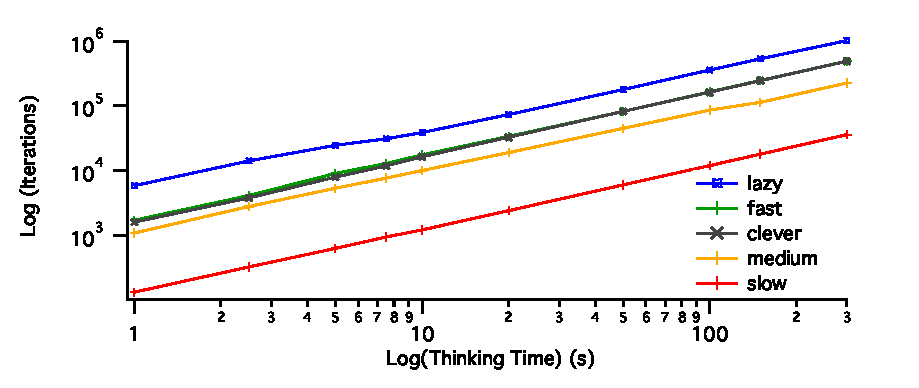
\includegraphics{thinking2.eps}}
\caption{Number of {MCTS} iterations performed to decide first move when starting from an empty $12\times 12$ board. Plotted against thinking time.}
\label{fig:linear}
\end{figure}

Figure \ref{fig:linear} shows that the number of iterations performed on the first move is directly proportional to the thinking time allocated for the first move. This is unsurpring for the {Slow}, {Medium}, {Fast}, and {Clever} agents. For these agents, every iteration represents performing a full Simulation from a start node to termination. It is a surprising result for the {Lazy} agent. In the {Lazy} agent, as more Simulations are performed, the tree grows, but only a maximum of 10 nodes are simulated beyond the fringe of the tree. From this, one would expect that the number of iterations performed per unit thinking time would decrease as the tree grows in size. Figure \ref{fig:linear} shows that this effect does not occur, at least for trees containing up to a million nodes. This suggests the Selection and Backpropagation phases are not a significant contribution to overhead, when compared to the Simulation and Expansion phases. Profiling data generated by the {Lazy} agent supported these findings.

\begin{figure}
\centering
{\includegraphics{boardsizeiter.eps}}
\caption{Number of {MCTS} iterations performed in 10 seconds to decide first move when starting from an empty board. Plotted against board size.\label{fig:boardsize}}
\end{figure}

Figure \ref{fig:boardsize} shows that all agents are roughly the same for small board sizes. This is unsuprising since {MCTS} quickly builds the entire game tree when the state space is small. For example, in the case of $3 \times 3$ boards, after about 1000 iterations the full game tree is built, and the rest of the work performed by the agent is repeated Selection. The Selection phase is implemented in the same way for all of the agents. 

The number of iterations performed decreases dramatically for all agents as the board size increases. This is to be expected since increasing board size increases both the branching factor at each move and the average depth at which Simulations terminate. The {Lazy} agent is affected least by the board size since the average depth at which Simulations terminate is always 10, regardless of board size.

The points in Figure \ref{fig:boardsize} for the {Lazy}, {Fast}, {Clever}and {Medium} agents look unreliable since they don't appear to fit a curve well. Repeated trials showed that the standard deviations for all points were at most $0.1\%$ of their corresponding mean values. The slightly erratic behaviour may be due to the idiosyncrasies of different board-sizes. In Figure \ref{fig:boardsize}, on a board size of 12 the {Clever} and {Fast} agents perform almost the exact same number of iterations as each other when given 10 seconds thinking time. Figure \ref{fig:linear} shows that this observation holds across a range of thinking times for $12 \times 12$ boards. 

In general, the {Clever} agent performs almost as well as the {Fast} agent. This strongly suggests that the {WinSave} heuristic contributes very little to the overall overhead of the search.



\subsection{{Connect}(12,12,5,1,1) Tournament Performance}

\begin{figure}
\centering
{\includegraphics{slowwld.eps}}
{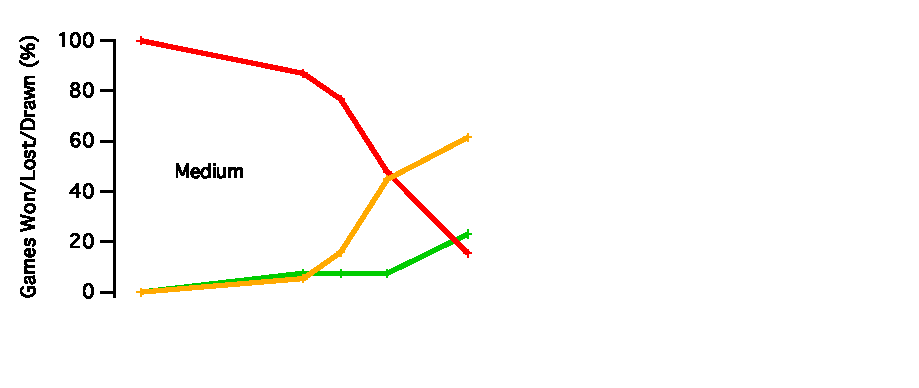
\includegraphics{medwld.eps}}
{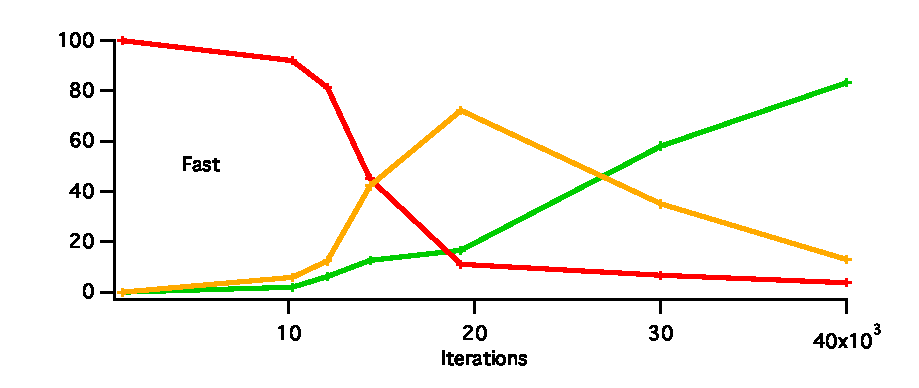
\includegraphics{fastwld.eps}}
\caption{Tournament results for the {Slow}, {Medium}, and {Fast} agents. Each plays against the {Threats} utility function with modest minimax search. The tournament results are plotted against the average number of iterations performed for the first move in each game.}
\label{fig:wld}
\end{figure}

Figure \ref{fig:wld} shows that, when the {Fast}, {Medium} and {Slow} agents are able to perform the same number of iterations on their first move, the three agents perform similarly in tournaments. This is consistent with the fact that {Fast}, {Medium} and {Slow} perform {MCTS} in exactly the same way, the only difference being their efficiency (see informal proof in Section \ref{sec:informal_proof}). The {Slow} and {Medium} agents are not plotted for the full $x$ axis due to Simulation time constraints. For example, a single 100 game tournament for the {Slow} agent for an $x$ value of 40,000, would take approximately 33 hours.

Figure \ref{fig:wld} also shows three approximate phases of tournament performance: for 0-15 thousand iterations, most games are lost; for 15-27 thousand iterations, most games are drawn; and for more than 27 thousand iterations, most games are won. Qualitive analysis of games played show two sub phases in the 0-15 thousand range: for 0-8 thousand iterations, most moves seem irrational and essentially random; for 8-15 thousand iterations, most moves are sensible but the agent is outplayed by the stronger {Threats} agent. 

\begin{figure}
\centering
{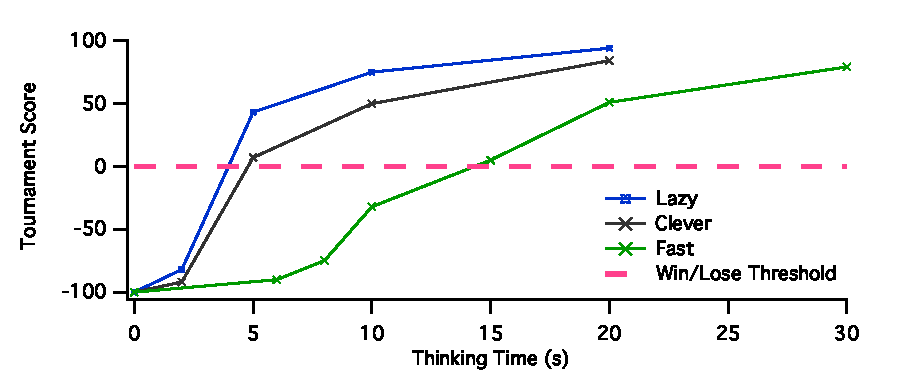
\includegraphics{thinking.eps}}
\caption{The tournament results plotted against thinking time.}
\label{fig:results}
\end{figure}

Figure \ref{fig:results} shows that, for any given thinking time, the most successful agents are {Lazy}, {Clever} and {Fast} in that order. {Slow} and {Medium} are not considered as they perform {MCTS} in the same fashion as {Fast}, but at a slower speed. The fact that {Clever} performs better than {Fast} is to be expected; the {WinSave} heuristic has runtime performance almost as good as {Fast}, but has a more rational tree and Simulation policy. The fact that {Lazy} performs better than {Clever} is interesting: for $12 \times 12$ boards, the boost in speed performance from terminating Simulations early outweighs the loss in tournament performance per iteration. Figure \ref{fig:boardsize} suggests that as boards get larger, the advantages of using {Lazy} over {Clever} increase.



\subsection{{Connect}(13,13,6,2,1) Tournament Performance}
No agents are able to play {Connect}(13,13,6,2,1) well against the {Threats} utility function, even when given up to 300 seconds thinking-time for each turn. The {Clever} agent is able to perform reasonably well against a random agent. However qualitive analysis of these games show that the {Clever} agent will play randomly until a win that turn is possible, or it is forced to block that turn. These results could be due to the high branching factor of {Connect}(13,13,6,2,1), $\binom{13 \times 13 -1}{2} = 20856$. This is about 145 times higher than the branching factor for {Connect}(12,12,5,1,1). The {Lazy} agent, which performs one million iterations in 300 seconds, would only be able to dedicate an average of 50 iterations to each of the possible moves within this time. This problem was foreseen during development, and as such, each ply of the game tree does not represent a single turn, but a single move. This reduces the branching factor in the tree to the `move' branching factor, 169. This result shows that this was not sufficient to solve the problem.

\subsection{{Freestyle GoMoku} and {Connect6} Tournaments}
The {Lazy} agent was chosen for the {Freestyle GoMoku} tournament since it outplays {Clever} for $12 \times 12$ boards. The number of iterations performed by {Lazy} on $15 \times 15$ boards is a slight increase on $12 \times 12$ boards. In contrast, the number of iterations performed by {Clever} from $12 \times 12$ to $15 \times 15$ boards drops by $40\%$. 

The tournament was played against the \text{Threats} utility function with modest search parameters. The {Lazy} agent won the tournament, winning $31\%$ of the games. The narrow margin of this win highlights the scalability issues for the {MCTS} agent. While the tournament performance of {Threats} with minimax search is fairly constant as board size increases, the performance of the {MCTS} agent deteriorates rapidly. Not only can fewer iterations be performed on larger boards, but more iterations are required to play well. It was not considered worthwhile running a {Connect6} tournament.

%Figure \ref{fig:wld}, \r shows this agent is fairly hopeless. The results for 100 seconds of thinking time are promising since it suggests there is nothing fundamentally wrong with the agent, but it needs to be made faster. Indeed, qualitative analysis shows game strategy gradually improves as more thinking time is permitted per move. The number of iterations performed increases linearly with thinking time. This suggests the main bulk of the work done in the {Simulation} phase and not the tree phases of the search. This is consistent with the profiling data gathered for this agent.

%Figure \ref{fig:slow313} shows the number of simulations which can be performed is inversely proportional to the ...










\cleardoublepage
\chapter{Conclusions}
In this project, an MCTS library and Connect agent were successfully implemented in Haskell.
\subsubsection{The library...}
\begin{itemize}
\item[] Can be used to implement a large range of games, from single-player puzzles to $n$-player, imperfect information, non-zero-sum, simultaneous play games.
\item[] Allows bespoke customization of the phases of {MCTS} described in the report while providing sensible defaults.
\item[] Supports the implementation of many of the modifications to {MCTS} proposed in current research.
\item[] Is user-friendly and fully documented (see Appendix \ref{sec:docs}).
\end{itemize}

\subsubsection{The {Connect} agent...}
\begin{itemize}
\item[] Can play any game in the {Connect} family.
\item[] Plays in a tactical fashion, akin to humans and other computer players, rather than strategically.
\item[] Beat a minimax-based agent in a 100-game {Freestyle GoMoku} tournament.
\item[] Is unable to play {Connect6} games to a good standard.
\end{itemize}
The use of Haskell in this project has been a pleasure. Despite the considerable investment in increasing code efficiency, there are significant advantages to using the language:
\begin{itemize}
\item[] Functional languages strongly resemble pure mathematics. This often makes the step of converting a mathematical definition of a function into an implementation in code straight-forward.
\item[] Functional languages are well-suited to test-driven development. It is a clean practice which allows function specifications to be embedded into the code.
\item[] Haskell supports features such as ad-hoc polymorphism and monadic programming. This makes it better suited to software engineering projects than other functional languages.
\item[] Very little time was required to debug code; most bugs were caught by the type-checker during compilation. Bugs that slipped the net usually led to failed QuickCheck properties.
\end{itemize}
The use of MCTS in this project has been interesting. It is fascinating that a search based upon random simulations and limited domain knowledge can perform well for such a diverse range of problems. It also posed a range of challenging problems during implementation. 

Connect was a poor choice for an example agent for the MCTS library. The game was chosen for the large state space and high branching factor, properties which are shared with {Go}. However, while it is difficult to write an effective utility function for Go, this is not the case for what {Connect}. Although {Go} has simple rules, the emergent complexity is profound. Gelly \& Silver \cite{go} noted that a move made now may not have an effect until 50 or 100 moves later. It was my hope that I might have revealed some of this complexity in {Connect}, but I suspect that most of the time spent simulating these distant scenarios was wasted. This is supported by the fact that the {Lazy} agent performed well, even though it did not run Simulations through to completion. 

A successful {MCTS} agent for {Connect6} has been constructed \cite{connect6}. However, it employs a large amount of domain specific knowledge. I wanted this example agent to remain agnostic to the specific human tactics of the game. An attempt to implement an agent for a more complex game, such as Kriegspiel, may have been a more suitable endeavour.



\cleardoublepage


%%%%%%%%%%%%%%%%%%%%%%%%%%%%%%%%%%%%%%%%%%%%%%%%%%%%%%%%%%%%%%%%%%%%%
% the bibliography

\addcontentsline{toc}{chapter}{Bibliography}
\bibliographystyle{plain}
\bibliography{main}
\cleardoublepage

%%%%%%%%%%%%%%%%%%%%%%%%%%%%%%%%%%%%%%%%%%%%%%%%%%%%%%%%%%%%%%%%%%%%%
% the appendices
\appendix
\chapter{Profiling Data}\label{app:profiling}
The following is raw profiling data generated by \textit{GHC}. The conclusion was made that the \texttt{doSimulation} function should be replaced with a more efficient implementation.
\begin{tiny}
\begin{verbatim}
Fri Mar  2 13:25 2012 Time and Allocation Profiling Report  (Final)

Main +RTS -p -RTS 
[[Nothing,Nothing,Nothing,Nothing,Nothing,Nothing], 
 [Nothing,Nothing,Nothing,Nothing,Nothing,Nothing], 
 [Nothing,Nothing,Nothing,Nothing,Nothing,Nothing],
 [Nothing,Nothing,Nothing,Nothing,Nothing,Nothing],
 [Nothing,Nothing,Nothing,Nothing,Nothing,Nothing],
 [Nothing,Nothing,Nothing,Nothing,Nothing,Nothing]]

	total time  =       13.74 secs   (687 ticks @ 20 ms)
	total alloc = 6,535,097,376 bytes  (excludes profiling overheads)

COST CENTRE                    MODULE               %time %alloc

doSimulation                   MCTS.Game             34.8   53.7
row                            MCTS.Sample.Connectk  14.8    3.7
doSelection                    MCTS.Config           12.2   14.1
kDiag                          MCTS.Sample.Connectk   9.0    7.9
funs                           MCTS.Sample.Connectk   6.8    3.7
kInARow                        MCTS.Sample.Connectk   5.2    5.9
pick                           MCTS.Game              5.1    1.8
mcts                           MCTS                   3.8    4.8
firstMatch                     MCTS.Sample.Connectk   2.8    0.0
averageScore                   MCTS                   1.5    1.3
topMcts                        MCTS                   1.0    1.8


                                                                                               individual    inherited
COST CENTRE              MODULE                                               no.    entries  %time %alloc   %time %alloc

MAIN                     MAIN                                                   1           0   0.0    0.0   100.0  100.0
 main                    Main                                                 568           3   0.0    0.0   100.0  100.0
  cmpBoard               Main                                                 654           3   0.0    0.0     0.0    0.0
   cmpRow                Main                                                 655           4   0.0    0.0     0.0    0.0
  iterativeMcts          MCTS.Mcts                                            574      369964   0.6    0.2    99.6   99.3
   topMcts               MCTS.Mcts                                            581       20000   1.0    1.8    99.0   99.1
    doBackpropagation    MCTS.Mcts                                            614       10000   0.0    0.0     0.0    0.0
    rChildList           MCTS.Mcts                                            596      730000   0.1    0.0     0.1    0.0
    doSelection          MCTS.Mcts                                            595      370000   3.6    4.1     4.9    4.8
     averageScore        MCTS.Mcts                                            604           0   0.9    0.5     1.0    0.5
      rQ                 MCTS.Mcts                                            627      359299   0.1    0.0     0.1    0.0
      rPlayed            MCTS.Mcts                                            605      359999   0.0    0.0     0.0    0.0
     rPlayed             MCTS.Mcts                                            603           0   0.3    0.1     0.3    0.1
    mcts                 MCTS.Mcts                                            591       33834   3.8    4.8    92.1   91.8
     doBackpropagation   MCTS.Mcts                                            634       23521   0.3    0.0     0.3    0.0
      rQ                 MCTS.Mcts                                            636       23360   0.0    0.0     0.0    0.0
      rPlayed            MCTS.Mcts                                            635       23521   0.0    0.0     0.0    0.0
     doSelection         MCTS.Mcts                                            630      838466   8.6   10.0     9.9   11.0
      rPlayed            MCTS.Mcts                                            633           0   0.4    0.3     0.4    0.3
      averageScore       MCTS.Mcts                                            631           0   0.6    0.8     0.9    0.8
       rQ                MCTS.Mcts                                            637      511062   0.3    0.0     0.3    0.0
       rPlayed           MCTS.Mcts                                            632      814632   0.0    0.0     0.0    0.0
     rChildList          MCTS.Mcts                                            629           0   0.1    0.0     0.1    0.0
     simulateNode        MCTS.Mcts                                            613       10000   0.0    0.0    73.1   73.4
      doBackpropagation  MCTS.Mcts                                            625        7577   0.0    0.0     0.0    0.0
       rQ                MCTS.Mcts                                            628        7531   0.0    0.0     0.0    0.0
       rPlayed           MCTS.Mcts                                            626        7577   0.0    0.0     0.0    0.0
      simulate           MCTS.Mcts                                            616      207640  34.8   53.7    73.1   73.4
       pick              Game.Game                                            623      197640   5.1    1.8     5.1    1.8
       kDiag             Game.Connectk                                        621     1609188   7.7    6.4    13.2    9.5
        funs             Game.Connectk                                        622      804594   5.5    3.1     5.5    3.1
       kInARow           Game.Connectk                                        618     1214111   4.4    4.9    19.2    8.5
        row              Game.Connectk                                        620    38748590  13.1    3.6    13.1    3.6
        firstMatch       Game.Connectk                                        619     8457967   1.7    0.0     1.7    0.0
       firstMatch        Game.Connectk                                        617     1411816   0.7    0.0     0.7    0.0
      rGame              MCTS.Mcts                                            615           0   0.0    0.0     0.0    0.0
     rPlayed             MCTS.Mcts                                            612       33834   0.1    0.0     0.1    0.0
     kDiag               Game.Connectk                                        610      270672   1.2    1.1     2.2    1.6
      funs               Game.Connectk                                        611      135336   1.0    0.5     1.0    0.5
     kInARow             Game.Connectk                                        594      203004   0.9    0.8     2.6    0.9
      row                Game.Connectk                                        607     6496128   1.5    0.1     1.5    0.1
      firstMatch         Game.Connectk                                        606     1421028   0.3    0.0     0.3    0.0
     firstMatch          Game.Connectk                                        593      236838   0.0    0.0     0.0    0.0
     rGame               MCTS.Mcts                                            592           0   0.0    0.0     0.0    0.0
    kDiag                Game.Connectk                                        587       80000   0.1    0.3     0.4    0.5
     funs                Game.Connectk                                        588       40000   0.3    0.2     0.3    0.2
    kInARow              Game.Connectk                                        584       60000   0.0    0.2     0.3    0.2
     row                 Game.Connectk                                        586     1920000   0.3    0.0     0.3    0.0
     firstMatch          Game.Connectk                                        585      420000   0.0    0.0     0.0    0.0
    firstMatch           Game.Connectk                                        583       70000   0.0    0.0     0.0    0.0
    rGame                MCTS.Mcts                                            582           0   0.0    0.0     0.0    0.0
   rChildList            MCTS.Mcts                                            575       20000   0.0    0.0     0.0    0.0
  expand                 MCTS.Mcts                                            573       90602   0.4    0.6     0.4    0.6
   rGame                 MCTS.Mcts                                            576           1   0.0    0.0     0.0    0.0
  gameToLeaf             MCTS.Mcts                                            572           1   0.0    0.0     0.0    0.0
  playerList             Game.Connectk                                        571           1   0.0    0.0     0.0    0.0
  selectBestMove         MCTS.Mcts                                            569           1   0.0    0.0     0.0    0.0
   rGame                 MCTS.Mcts                                            649           1   0.0    0.0     0.0    0.0
   averageScore          MCTS.Mcts                                            641           0   0.0    0.0     0.0    0.0
    rQ                   MCTS.Mcts                                            643          70   0.0    0.0     0.0    0.0
    rPlayed              MCTS.Mcts                                            642          70   0.0    0.0     0.0    0.0
   rChildList            MCTS.Mcts                                            570           2   0.0    0.0     0.0    0.0
 CAF:lvl14_ro80          Main                                                 562           1   0.0    0.0     0.0    0.0
 CAF:lvl13_ro7Y          Main                                                 561           1   0.0    0.0     0.0    0.0
  main                   Main                                                 578           0   0.0    0.0     0.0    0.0
 CAF:lvl12_ro7W          Main                                                 560           1   0.0    0.0     0.0    0.0
  main                   Main                                                 579           0   0.0    0.0     0.0    0.0
 CAF:lvl11_ro7U          Main                                                 559           1   0.0    0.0     0.0    0.0
  main                   Main                                                 580           0   0.0    0.0     0.0    0.0
 CAF:lvl10_ro7S          Main                                                 558           1   0.0    0.0     0.0    0.0
 CAF:lvl9_ro7Q           Main                                                 557           1   0.0    0.0     0.0    0.0
  main                   Main                                                 651           0   0.0    0.0     0.0    0.0
 CAF:lvl8_ro7O           Main                                                 556           1   0.0    0.0     0.0    0.0
  main                   Main                                                 652           0   0.0    0.0     0.0    0.0
 CAF:lvl7_ro7M           Main                                                 555           1   0.0    0.0     0.0    0.0
  main                   Main                                                 653           0   0.0    0.0     0.0    0.0
 CAF:$dEq_ro7I           Main                                                 554           1   0.0    0.0     0.0    0.0
 CAF                     GHC.Read                                             532           2   0.0    0.0     0.0    0.0
 CAF                     GHC.Float                                            531           1   0.0    0.0     0.0    0.0
 CAF                     Text.Read.Lex                                        520           5   0.0    0.0     0.0    0.0
 CAF                     GHC.Int                                              516           2   0.0    0.0     0.0    0.0
 CAF                     GHC.IO.Handle.FD                                     490           2   0.0    0.0     0.0    0.0
 CAF                     GHC.IO.Encoding.Iconv                                448           2   0.0    0.0     0.0    0.0
 CAF                     GHC.Conc.Signal                                      445           1   0.0    0.0     0.0    0.0
 CAF:lvl42_r9vn          MCTS.Mcts                                            437           1   0.0    0.0     0.0    0.0
  selectBestMove         MCTS.Mcts                                            638           0   0.0    0.0     0.0    0.0
   averageScore          MCTS.Mcts                                            639           1   0.0    0.0     0.0    0.0
    rQ                   MCTS.Mcts                                            648           1   0.0    0.0     0.0    0.0
    rPlayed              MCTS.Mcts                                            640           1   0.0    0.0     0.0    0.0
 CAF:lvl41_r9vl          MCTS.Mcts                                            436           1   0.0    0.0     0.0    0.0
  selectBestMove         MCTS.Mcts                                            644           0   0.0    0.0     0.0    0.0
   averageScore          MCTS.Mcts                                            645           1   0.0    0.0     0.0    0.0
    rQ                   MCTS.Mcts                                            647           1   0.0    0.0     0.0    0.0
    rPlayed              MCTS.Mcts                                            646           1   0.0    0.0     0.0    0.0
 CAF:lvl40_r9ve          MCTS.Mcts                                            435           1   0.0    0.0     0.0    0.0
  doSelection            MCTS.Mcts                                            600           0   0.0    0.0     0.0    0.0
   averageScore          MCTS.Mcts                                            601           1   0.0    0.0     0.0    0.0
    rPlayed              MCTS.Mcts                                            602           1   0.0    0.0     0.0    0.0
 CAF:$dNum_r9uU          MCTS.Mcts                                            431           1   0.0    0.0     0.0    0.0
 CAF:lvl35_r9uk          MCTS.Mcts                                            428           1   0.0    0.0     0.0    0.0
 CAF:lvl34_r9ui          MCTS.Mcts                                            427           1   0.0    0.0     0.0    0.0
 CAF                     System.Random                                        393           1   0.0    0.0     0.0    0.0
 CAF                     Data.Fixed                                           388           3   0.0    0.0     0.0    0.0
 CAF                     Data.Time.Clock.POSIX                                385           2   0.0    0.0     0.0    0.0
 CAF:lvl6_rkVC           Game.Connectk                                        301           1   0.0    0.0     0.0    0.0
  row                    Game.Connectk                                        624           0   0.0    0.0     0.0    0.0
 CAF:lvl5_rkVA           Game.Connectk                                        300           1   0.0    0.0     0.0    0.0
  row                    Game.Connectk                                        608           0   0.0    0.0     0.0    0.0
 CAF:k                   Game.Connectk                                        299           1   0.0    0.0     0.0    0.0
  k                      Game.Connectk                                        609           1   0.0    0.0     0.0    0.0
 CAF:funs2               Game.Connectk                                        297           1   0.0    0.0     0.0    0.0
  funs                   Game.Connectk                                        589           0   0.0    0.0     0.0    0.0
 CAF:lvl4_rkVu           Game.Connectk                                        296           1   0.0    0.0     0.0    0.0
  funs                   Game.Connectk                                        590           0   0.0    0.0     0.0    0.0
  \end{verbatim}
  \end{tiny}

\end{document}